\section{The Determinants of the Aggregate Market Elasticity}\label{sec:elasticity}

% In this section, we analyze how the \textit{aggregate market elasticity} shapes how portfolio flows affect asset prices. 
% The elasticity is determined by the coupled PDE system \eqref{eq:xi_j}–\eqref{eq:pricing_cond}, which generally admits no closed-form solution. 
% To understand its determinants, we extend the perturbation method of \citet{kogan2001risk} and derive asymptotic closed-form expressions for the elasticity.
In this section, we analyze how the \emph{aggregate market elasticity} governs the price impact of portfolio flows.  
The elasticity is determined by the coupled PDE system \eqref{eq:xi_j}–\eqref{eq:pricing_cond}, which generally has no closed-form solution. To study its determinants, we extend the perturbation method of \citet{kogan2001risk} and derive asymptotic closed-form approximations.

\paragraph{State-global perturbations}

Our perturbation approach studies economies in a neighborhood of a benchmark that admits a closed-form solution.
% A convenient benchmark consists of the case where there is no preference heterogeneity, $\gamma_j = \gamma$, and passive investors are fully invested in the risky asset, $\overline{\alpha}_{p,t} = 1$. 
% In this case, we effectively obtain a Lucas economy, as shown in the next lemma. 
% Throughout, a superscript $*$ denotes the benchmark economy.
A convenient benchmark arises when preferences are homogeneous, $\gamma_j=\gamma$, and passive investors are fully invested in the risky asset, $\overline{\alpha}_{p,t}=1$. In this case, the economy collapses to a Lucas economy, as shown in Lemma~\ref{lemma:benchmark}. Throughout, a superscript $*$ denotes benchmark values.



\begin{lemma}[Benchmark economy]\label{lemma:benchmark}
Suppose $\gamma_j = \gamma$, $\overline{\alpha}_{p,t} = 1$, and $\rho>\big(1-\psi^{-1}\big)\big(\mu - \frac{\gamma \|\sigma\|^2}{2}\big)$. Then, 
\begin{equation}
        \pi^* = \gamma \|\sigma\|^2, \qquad 
        r^* = \rho + \psi^{-1}\mu - \big(1+\psi^{-1}\big)\frac{\gamma \|\sigma\|^2}{2}, \qquad 
        p^* = \Big[\rho - \big(1-\psi^{-1}\big)\Big(\mu - \frac{\gamma \|\sigma\|^2}{2}\Big)\Big]^{-1},
\end{equation}
$c_{j}^* = (p^*)^{-1}$, and $\alpha_{j}^* = 1$ for $j = 0, \ldots, J$.
\end{lemma}

We analyze small deviations from this benchmark. Formally, consider a family of economies indexed by $\epsilon>0$, where $\epsilon$ scales departures from the benchmark along the following dimensions.

First, investors have heterogeneous risk aversion:
\begin{equation}\label{eq:gamma-perturb}
    \gamma_j=\gamma\big(1+\hat{\gamma}_j\epsilon\big), 
    \qquad
    \sum_{j=0}^J \omega_j \hat{\gamma}_j=0,
\end{equation}
so that $\gamma$ is the population-weighted average and $\hat{\gamma}_j$ measures deviations. When $\epsilon=0$, preferences are homogeneous; when $\epsilon=1$, we recover the heterogeneous-investor economy.

% Second, passive investors need not be fully invested in the risky asset. We write their portfolio share as  
% \begin{equation}\label{eq:apbar_index}
%     \overline{\alpha}_{p,t} \;=\; 1 + \hat{\alpha}_{p,t}\,\epsilon,
% \end{equation}
% where $\hat{\alpha}_{p,t}$ captures deviations from the benchmark of full investment and evolves according to an Ornstein-Uhlenbeck process, consistent with Equation~\eqref{eq:alpha_p_process}.% Second, the passive investor may not be fully invested in the risky asset:
% \begin{equation}\label{eq:apbar_index}
%     \overline{\alpha}_{p,t}=1+\hat{\alpha}_{p,t}\,\epsilon,
% \end{equation}
% where $\hat{\alpha}_{p,t}$, which governs deviations from the benchmark, follows an Ornstein-Uhlenbeck process, consistent with Equation~\eqref{eq:alpha_p_process}. 

% For simplicity, we abstract from time variation in passive portfolios and take $\hat{\alpha}_p$ as constant. In this case $Z_t$ is one-dimensional and we set $\sigma\equiv\|\sigma\|$.

Second, passive investors need not be fully invested in the risky asset. Their portfolio share is  
\begin{equation}\label{eq:apbar_index}
    \overline{\alpha}_{p,t}=1+\hat{\alpha}_{p,t}\,\epsilon,
\end{equation}
where $\hat{\alpha}_{p,t}$ measures deviations from full investment benchmark and evolves as an Ornstein-Uhlenbeck process, consistent with Equation~\eqref{eq:alpha_p_process}.

% We also assume the leverage-constraint coefficient satisfies
% \begin{equation}\label{eq:sig_bar-perturb}
%     \overline{\sigma}=\sigma\left(1+\hat{\sigma}\,\epsilon\right),
% \end{equation}
% so that the tightness of the constraint is $\mathcal{O}(\epsilon)$, matching the order of leverage demand. Finally, we assume the mortality parameter is small: $\kappa=\hat{\kappa}\,\epsilon$.

Third, the leverage constraint coefficient is perturbed according to
\begin{equation}\label{eq:sig_bar-perturb}
    \overline{\sigma}=\|\sigma\|\big(1+\hat{\sigma}\,\epsilon\big),
\end{equation}
so that the tightness of the constraint is of order $\mathcal{O}(\epsilon)$, matching the order of leverage demand. Finally, we assume a small mortality rate, $\kappa=\hat{\kappa}\,\epsilon$.

% Equilibrium objects now depend on both the state $X_t$ and the parameter $\epsilon$. We expand them to second order in $\epsilon$:
% \begin{align}
%     p(X,\epsilon) &= p_0(X) + p_1(X)\epsilon + p_2(X)\epsilon^2 + \mathcal{O}(\epsilon^3), \\
%     c_j(X,\epsilon) &= c_{j,0}(X) + c_{j,1}(X)\epsilon + c_{j,2}(X)\epsilon^2 + \mathcal{O}(\epsilon^3),
% \end{align}
% where $p_k(X)$ and $c_{j,k}(X)$, $k\in \{0,1,2\}$, are functions of the state $X$.  

% Unlike standard DSGE perturbations, which linearize in both $X$ and $\epsilon$, our method is \emph{state-global}: we solve directly for functions of $X$ rather than local coefficients around a steady state.\footnote{A formal comparison with standard perturbation methods is provided in \citet{kargar2020competitive}.}
% We refer to this approach as a \textit{state-global perturbation}.\footnote{The method follows the perturbation approach of \citet{kogan2001risk} and builds on the extension of \citet{Silva/riskchannel} to economies with passive investors.}
% This allows us to characterize how the aggregate market elasticity varies with the state of the economy.

% We proceed in two steps: first, we characterize the first-order corrections $p_1(X)$ and $c_{j,1}(X)$; second, we solve for the second-order terms $p_2(X)$ and $c_{j,2}(X)$. The zeroth-order terms $p_0(X)$ and $c_{j,0}(X)$ are given by Lemma~\ref{lemma:benchmark}, that is, $p_0(X) = p^*$ and $c_{j,0}(X) = c_j^*$.
Equilibrium objects now depend on both the state $X_t$ and the parameter $\epsilon$. We expand them to second order:
\begin{align}
    p(X,\epsilon) &= p_0(X) + p_1(X)\epsilon + p_2(X)\epsilon^2 + \mathcal{O}(\epsilon^3), \\
    c_j(X,\epsilon) &= c_{j,0}(X) + c_{j,1}(X)\epsilon + c_{j,2}(X)\epsilon^2 + \mathcal{O}(\epsilon^3),
\end{align}
where $p_k(X)$ and $c_{j,k}(X)$, $k\in\{0,1,2\}$, are functions of the state $X$.

Unlike standard DSGE perturbations, which linearize in both $X$ and $\epsilon$, our method is \emph{state-global}: we solve directly for functions of $X$ rather than coefficients around a steady state.\footnote{See \citet{kargar2020competitive} for a comparison with standard perturbation methods.} 
We refer to this approach as a \emph{state-global perturbation}. 
This approach builds on the perturbation method of \citet{kogan2001risk} and, more closely, the extension 
by \citet{Silva/riskchannel}.
This method allows us to characterize how aggregate market elasticity varies with the state of the economy.

We proceed in two steps. First, we compute the first-order corrections $p_1(X)$ and $c_{j,1}(X)$. Second, we solve for the second-order terms $p_2(X)$ and $c_{j,2}(X)$. Zeroth-order terms are given by Lemma~\ref{lemma:benchmark}, i.e., $p_0(X)=p^*$ and $c_{j,0}(X)=c_j^*$.


% \subsubsection{The benchmark economy}

% In the absence of preference heterogeneity, and with passive investors fully invested in the risky asset, the economy effectively behaves as the frictionless Lucas economy with a representative agent. 

% \begin{lemma}[Benchmark economy]\label{lemma:benchmark}
% Suppose $\rho>\left(1-\psi^{-1}\right)\left( \mu - \frac{\gamma
% \sigma^2}{2}  \right)$.\footnote{The condition $\rho>\left(1-\psi^{-1}\right)\left( \mu - \frac{\gamma
% \sigma^2}{2}  \right)$ is standard in economies with growth and risk, guaranteeing that investors achieve finite utility.} Then, for the $\epsilon=0$ economy, 
% \begin{enumerate}[(i)]
% \item Investors' consumption-wealth ratio and risk exposure are given by:
% \begin{equation}
%  c_{j,0}(X) = \rho - \left(1-\psi^{-1}\right) \left( \mu - \frac{\gamma \sigma^2}{2} \right), \qquad \alpha_{j,0}(X) = 1, \qquad \text{for } j = 0,1,\ldots, J.\nonumber
% \end{equation}

% \item Risk premium, risk-free rate, and price-dividend ratio are given by:
% \begin{equation}\nonumber
%     \pi_0 (X) = \gamma \sigma^2, \qquad 
%     r_0(X) = \rho + \psi^{-1} \mu - \left (1+\psi^{-1}\right ) \frac{\gamma \sigma^2}{2}, \qquad 
%     p_0(X) =  \frac{1}{c_{j,0}(X)}.
% \end{equation}
% \end{enumerate}
% \end{lemma}
% \begin{proof}
% See Appendix~\ref{app:lemma1}.
% \end{proof}

% Lemma~\ref{lemma:benchmark} shows that there is no time variation in the expected returns in the benchmark economy in the absence of frictions. 
% In particular, the price-dividend ratio $p_0(X)$ is constant in the benchmark economy, so the risk premium and interest rate are given by the standard Lucas economy formulae.
% % Moreover, the return volatility is equal to the volatility of dividends since the price-dividend ratio $p_0(X)$ is constant in this case.

% \paragraph{The benchmark economy.}

% When preferences are homogeneous and passive investors are fully invested in the risky asset ($\epsilon=0$), the economy reduces to the frictionless Lucas representative-agent benchmark.  

% \begin{lemma}[Benchmark economy]\label{lemma:benchmark}
% Suppose $\rho>\big(1-\psi^{-1}\big)\big(\mu - \frac{\gamma \sigma^2}{2}\big)$,\footnote{This condition is standard in models with growth and risk and ensures finite utility.} then in the $\epsilon=0$ economy:
% \begin{enumerate}[(i)]
%     \item Consumption–wealth ratios and portfolio shares are
%     \[
%         c_{j,0}(X) = \rho - \big(1-\psi^{-1}\big)\Big(\mu - \frac{\gamma \sigma^2}{2}\Big), 
%         \qquad \alpha_{j,0}(X) = 1, 
%         \qquad j=0,1,\ldots,J.
%     \]
%     \item Risk premium, interest rate, and price–dividend ratio are
%     \[
%         \pi_0(X) = \gamma \sigma^2, \qquad 
%         r_0(X) = \rho + \psi^{-1}\mu - \big(1+\psi^{-1}\big)\frac{\gamma \sigma^2}{2}, \qquad 
%         p_0(X) = \frac{1}{c_{j,0}(X)}.
%     \]
% \end{enumerate}
% \end{lemma}
% \begin{proof}
% See Appendix~\ref{app:lemma1}.
% \end{proof}

% Lemma~\ref{lemma:benchmark} implies that in the absence of frictions, expected returns are constant: the price–dividend ratio $p_0(X)$ is fixed, and the risk premium and interest rate coincide with the standard Lucas economy formulas.


% \subsection{The first-order demand system}

% We consider next the first-order approximation of the demand system. 
% Investor $j$'s demand for the risky asset is given by $Q_{j}(X;\epsilon) = \alpha_{j}(X;\epsilon) \frac{x_{j}}{\omega_{j}}.$ 
% Let $q_{j,t} = \log Q_{j,t} / Q_{j,0}(X_t)$ denote the log deviation of investor $j$'s demand from her demand in the benchmark economy. Up to first order, we can write $q_{j,t}$ as follows:
% \begin{equation}
%     q_{j,t} = \alpha_{j,1}(X_t) \epsilon + \mathcal{O}(\epsilon^2),
% \end{equation}
% where $\alpha_{j,1}(X_t) $ is the first-order correction for portfolio weight $\alpha_j(X;\epsilon)$. Three observations are important in computing $\alpha_{j,1}$. First, the endogenous volatility is equal to zero up to first order, as $\sigma_{p,t}$ is given by 
% \begin{equation}
%     \sigma_{p,t} = \frac{p_x(X_t)}{p(X_t)} \sigma_x(X_t) = \left[ \frac{p_{x,1}(X_t)}{p_0(X_t)} \sigma_{x,0}(X_t) +\frac{p_{x,0}(X_t)}{p_0(X_t)} \sigma_{x,1}(X_t) \right] \epsilon + \mathcal{O}(\epsilon^2) = \mathcal{O}(\epsilon^2),
% \end{equation}
% where $p_{x,0}(X_t) = \sigma_{x,0}(X_t) = 0$, as shown in Lemma \ref{lemma:benchmark}. Second, the hedging demand is also second-order in $\epsilon$, $\varsigma_{j,t} = \mathcal{O}(\epsilon^2)$,
% as a similar argument shows that $\sigma_{c_j}(X_t) = \mathcal{O}(\epsilon^2)$. Third, expanding the pricing condition \eqref{eq:pricing_cond}, we obtain the analogous of Equation \eqref{eq: risk_premium}:
% \begin{equation}
% \hat{\pi}_t = - \hat{r}_t - \frac{1}{p^*} \hat{p}_t + \mathcal{O}(\epsilon^2),
% \end{equation}
% where $\hat{\pi}_t \equiv \pi_t - \pi_0(X_t)$, $\hat{r}_t \equiv r_t - r_0(X_t)$, and $\hat{p}_t = \frac{p_t - p^*}{p^*}$, using the fact that $\mu_{p,t} = \mathcal{O}(\epsilon^2)$ and $p^* \equiv p_0(X)$. 
% As in Section \ref{sec:simple}, we can use the pricing condition to write the risk premium in terms of the price-dividend ratio and the interest rate.

% Using the three observations above, we can compute the first-order expansion of the portfolio share in Equation \eqref{eq:portfolio_share} to obtain investor $j$'s demand for an unconstrained investor :
% \begin{equation}\label{eq:demand_risky}
%     q_{j,t} = -\zeta^q_{j, p} \hat{p}_t - \zeta^q_{j,r} \hat{r}_t + f_{j,t} + \mathcal{O}(\epsilon^2), 
% \end{equation}
% where $$\zeta_{j,p}^q \equiv \frac{1}{p^*} \frac{1}{\gamma \sigma^2}, \qquad \zeta_{j,r}^q \equiv \frac{1}{\gamma \sigma^2}, \qquad f_{j,t} \equiv -\hat{\gamma}_j \epsilon.$$ 
% A similar equation holds for a constrained investor, but in this case $\zeta_{j,p}^q = \zeta_{j,r}^q = 0$ and $f_{j,t} = \frac{\hat{\sigma}}{\|\sigma\|} \epsilon$. 
% The demand from passive investors also takes the form above, with $\zeta_{0,p}^q = \zeta_{0,r}^q = 0$, and $f_{0,t} = \hat{\alpha}_{p} \epsilon$.

% The demand for the risky asset for unconstrained agents is analogous to the active demand in Section~\ref{sec:simple}. 
% However, we can now relate the elasticities to the underlying parameters. 
% The price elasticity $\zeta_{j,p}^q$ is given by $\frac{1/p^*}{\gamma \sigma^2}$, the ratio of the dividend yield and the risk premium in the benchmark economy, while the cross price-elasticity $\zeta_{j,r}^q$ is given by the inverse of the risk premium.  Importantly, the cross price-elasticity is non-zero for unconstrained investors. 
% As shown above, the direct and cross price elasticities are equal to zero for a constrained investor. 
% Finally, even if $\hat{r}_t = \hat{\pi}_t = 0$, investors' demand would deviate from the one in the benchmark economy due to differences in risk aversion, the leverage limit, or the passive portfolio. 
% These effects are captured by the demand shifters $f_{j,t}$.

% We can proceed in an analogous way to compute the first-order expansion of the consumption-wealth ratio in Equation~\eqref{eq:xi_j}:
% \begin{equation}
%     c_{j,t} = \psi \rho + (1-\psi) \left[ r_t + \pi_t  - \frac{\gamma_j \sigma^2}{2}  \right] + \mathcal{O}(\epsilon^2),
% \end{equation}
% where we used the fact that $\xi_t = \mathcal{O}(\epsilon^2)$. 
% % Consistent with Assumption \ref{assump:c_w_property}, the risk-free rate and the risk premium affect in the same way the consumption-wealth ratio up to first order. 
% In line with Assumption~\ref{assump:c_w_property}, both the risk-free rate and risk premium have a similar first-order impact on the consumption-wealth ratio.
% Using the pricing condition, we can write $\hat{c}_{j,t} \equiv c_{j,t} - c_{j,0}(X_t)$ in terms of $\hat{p}_t$ and a shifter:
% \begin{equation}
%     \hat{c}_{j,t} = \zeta^c_{j,p} \hat{p}_t + \zeta^c_{j,0},
% \end{equation}
% where $\zeta_{j,p}^c \equiv (\psi-1) \frac{1}{p^*}$ and $\zeta^c_{j,0} \equiv (\psi-1) \frac{\gamma \sigma^2}{2} \hat{\gamma}_j \epsilon$.
% Notice that the consumption-wealth ratio does not depend on $r_t$ given $p_t$, as in Section \ref{sec:simple}.
% The consumption-wealth ratio can be either increasing or decreasing in $p_t$.
% The case depicted in Figure \ref{fig:mkt_equilibrium}, where the consumption-wealth ratio is increasing in $p_t$, corresponds to $\psi > 1$, a common assumption in macro-finance models (see e.g. \citealt{bansal2004risks}).
% Another important property is that the consumption-wealth ratio is independent of $\overline{\alpha}_{p,t}$, which has implications for the determination of the market elasticity.


\subsection{The first-order demand system}

\paragraph{Demand for risky asset.}  
Investor $j$’s demand for the risky asset is 
\[
    Q_j(X;\epsilon)=\alpha_j(X;\epsilon)\,\frac{x_j}{\omega_j},
\]
where $x_j$ is the wealth share. Define the proportional deviation from the benchmark as
\begin{equation}
    q_{j,t}\;\equiv\;\frac{Q_j(X_t;\epsilon)- Q_j(X_t;0)}{Q_j(X_t;0)}
    \;=\;\alpha_{j,1}(X_t)\,\epsilon+\mathcal{O}(\epsilon^2),
\end{equation}
where $\alpha_{j,1}(X)$ is the first-order correction to the portfolio weight.  

Three results determine $\alpha_{j,1}(X)$. First, the volatility of the price-dividend ratio is second order:
\[
    \sigma_{p,t}=\frac{p_X(X_t)}{p(X_t)}\,\sigma_X(X_t)=\mathcal{O}(\epsilon^2),
\]
since $p_{X,0}=\sigma_{X,0}=0$ (Lemma~\ref{lemma:benchmark}). Second, hedging demand is also $\mathcal{O}(\epsilon^2)$ because $\sigma_{c_j}(X_t)$ is second order. Third, expanding the pricing condition \eqref{eq:pricing_cond} gives
\begin{equation}
    \hat{\pi}_t=-\,\hat{r}_t-\frac{1}{p^*}\hat{p}_t+\mathcal{O}(\epsilon^2),
\end{equation}
where $\hat{\pi}_t\equiv \pi_t-\pi^*$, $\hat{r}_t\equiv r_t-r^*$, and $\hat{p}_t\equiv \frac{p_t-p^*}{p^*}$, using $\mu_{p,t}=\mathcal{O}(\epsilon^2)$.

Substituting into \eqref{eq:portfolio_share}, the first-order demand system is
\begin{equation}\label{eq:demand_risky}
    q_{j,t}=-\,\zeta_{j,p}\,\hat{p}_t-\zeta_{j,r}\,\hat{r}_t+f_{j,t}+\mathcal{O}(\epsilon^2),
\end{equation}
where, for unconstrained investors,
\[
    \zeta_{j,p}=\frac{1}{p^*}\frac{1}{\gamma\|\sigma\|^2}, 
    \qquad
    \zeta_{j,r}=\frac{1}{\gamma\|\sigma\|^2}, 
    \qquad
    f_{j,t}=-\,\hat{\gamma}_j\,\epsilon.
\]
For passive and constrained investors, own- and cross-price elasticities vanish, $\zeta_{j,p}=\zeta_{j,r}=0$, with demand shifters $f_{j,t}=\hat{\sigma}\,\epsilon$ for constrained investors and $f_{0,t}=\hat{\alpha}_{p,t}\,\epsilon$ for passive investors.  

Equation~\eqref{eq:demand_risky} shows that the first-order approximation to the dynamic heterogeneous agent model in Section~\ref{sec:model} provides microfoundations for the demand system in Section~\ref{sec:simple}. As in the simple model, unconstrained active investors exhibit nonzero own- and cross-price elasticities, here explicitly linked to structural parameters. Shocks to $\overline{\alpha}_{p,t}$ move the passive investors’ demand shifter $f_{0,t}$—the dynamic analog of the comparative statics in Section~\ref{sec:simple}. In addition, the model generates further demand shifts from occasionally binding leverage constraints faced by active investors.

% \paragraph{Consumption-wealth ratio.}
% Similarly, the first-order expansion of \eqref{eq:xi_j} for consumption yields
% \begin{equation}
%     c_{j,t}
%     \;=\;
%     \psi\rho \;+\; (1-\psi)\!\left[r_t + \pi_t - \frac{\gamma_j\sigma^2}{2}\right]
%     \;+\; \mathcal{O}(\epsilon^2).
% \end{equation}
% In line with Assumption~\ref{assump:c_w_property}, the risk-free rate and the risk premium have the same first-order impact on the consumption–wealth ratio. Using the expansion
% \(\hat\pi_t = -\,\hat r_t - p^{*\, -1}\hat p_t + \mathcal{O}(\epsilon^2)\), we obtain
% \begin{equation}
%     \hat c_{j,t} \;\equiv\; c_{j,t} - c_{j}^*
%     \;=\; \chi_{j,0} \;+\; \chi_{j,p}\,\hat p_t \;+\; \mathcal{O}(\epsilon^2),
% \end{equation}
% with
% $    \chi_{j,p} \;\equiv\; (\psi-1)\,\frac{1}{p^*},$ 
%     and
%     $\chi_{j,0} \;\equiv\; (\psi-1)\,\frac{\gamma\sigma^2}{2}\,\hat{\gamma}_j\,\epsilon.
% $


% Hence, conditional on \(p_t\), the consumption–wealth ratio is independent of \(r_t\), as in Section~\ref{sec:simple}. Its slope with respect to \(p_t\) depends on the EIS: it is increasing in \(p_t\) when \(\psi>1\), as in standard macro-finance models \citep{bansal2004risks}. Finally, the consumption–wealth ratio is independent of \(\overline{\alpha}_{p,t}\) to first order, a fact that will matter for aggregate market elasticity.

\paragraph{Consumption-wealth ratio.}  
A first-order expansion of \eqref{eq:xi_j} yields
\begin{equation}
    c_{j,t}
    \;=\;
    \psi\rho \;+\; (1-\psi)\!\left[r_t + \pi_t - \frac{\gamma_j\|\sigma\|^2}{2}\right]
    \;+\; \mathcal{O}(\epsilon^2).
\end{equation}
Consistent with Assumption~\ref{assump:c_w_property}, the risk-free rate and the risk premium enter symmetrically at first order. Substituting the expansion
\(\hat{\pi}_t = -\,\hat{r}_t - p^{*\,-1}\hat{p}_t + \mathcal{O}(\epsilon^2)\) gives
\begin{equation}
    \hat c_{j,t} \;\equiv\; c_{j,t} - c_j^*
    \;=\; \chi_{j,0} \;+\; \chi_{j,p}\,\hat{p}_t \;+\; \mathcal{O}(\epsilon^2),
\end{equation}
with coefficients
\[
    \chi_{j,p}=(\psi-1)\,\frac{1}{p^*},
    \qquad 
    \chi_{j,0}=(\psi-1)\,\frac{\gamma\|\sigma\|^2}{2}\,\hat{\gamma}_j\,\epsilon.
\]

Hence, conditional on $p_t$, the consumption-wealth ratio is independent of $r_t$, as in Section~\ref{sec:simple}. Its slope with respect to $p_t$ depends on the EIS: it rises with $p_t$ when $\psi>1$, the standard assumption in macro-finance models. Finally, to first order, the consumption–wealth ratio is unaffected by $\overline{\alpha}_{p,t}$, a property that will be central for aggregate market elasticity.

% \subsubsection{Aggregate market elasticity in frictionless economies}

% Given the demand system, we can solve for the equilibrium prices. The market clearing conditions for the risky asset and for goods can be written as
% \begin{equation}
%     \sum_{j=0}^J x_{j} q_{j,t} = 0, \qquad \qquad 
%     \sum_{j=0}^J x_{j} \hat{c}_{j,t} = -\frac{1}{p^*} \hat{p}_t,\nonumber
% \end{equation}

% Aggregating the demand for the risky asset and the consumption-wealth ratio, we obtain
% \begin{equation}
%     \left[
%     \begin{matrix}
%         \zeta^q_p & \zeta^q_r\\
%         \zeta^c_p + \frac{1}{p^*} & 0
%     \end{matrix}
%     \right]\left[ \begin{matrix}
%         \hat{p}_t\\
%         \hat{r}_t
%     \end{matrix} \right] =
%     \left[ \begin{matrix}
%         f_t\\
%         -\zeta_{0}^c
%     \end{matrix} \right],\nonumber
% \end{equation}
% where $\zeta^q_{k} \equiv \sum_{j=0}^J x_j \zeta_{j,k}^q$, for $k \in \{p,r\}$, $\zeta^c_{k} \equiv \sum_{j=0}^J x_j \zeta^c_{j,k}$, for $k \in \{p,0\}$, and $f_t \equiv \sum_{j=0}^J x_j f_{j,t}$.

% Solving the system above, we obtain asset prices in this economy: 
% \begin{equation}
%     \hat{p}_t = - \frac{\zeta_0^c}{\zeta_p^c + \frac{1}{p^*} }, \qquad \qquad 
%     \hat{r}_t = \frac{f_t}{\zeta_r^q} + \frac{\zeta_p^q}{\zeta_r^q \left( \zeta_p^c + \frac{1}{p^*} \right)} \zeta_0^c.\nonumber
% \end{equation}

% The aggregate market elasticity, $\epsilon_{M,t}$, is defined as the inverse of the proportional change in the price of the risky asset in response to a portfolio flow shock $f_t$:
% \begin{equation}
%     \epsilon_{M,t}^{-1} = \left( \frac{\partial \hat{p}_t}{\partial f_t} \right)^{-1}.\nonumber
% \end{equation}

% As $\hat{p}_t$ is independent of the portfolio flow shock $f_t$, the inverse elasticity is equal to zero up to first order:
% \begin{equation}
%     \epsilon_{M,t}^{-1} = 0.
% \end{equation}
% This result echoes the findings in Section \ref{sec:simple} which showed how the aggregate elasticity could be infinite in the context of a two-period economy. We obtain the same result now in the context of our dynamic economy using a first-order approximation.

\paragraph{Aggregate market elasticity.}  
Given the demand system, equilibrium prices follow from market clearing in the risky-asset and goods markets:
\[
    \sum_{j=0}^J x_{j,t}\, q_{j,t} = 0,
    \qquad
    \sum_{j=0}^J x_{j,t}\, \hat{c}_{j,t} = -\frac{1}{p^*}\,\hat{p}_t .
\]

Aggregating across investors, and dropping the $j$ subscript on coefficients that are common across types, yields the linear system
\[
    \begin{bmatrix}
        \zeta_p & \zeta_r \\
        \chi_p + \tfrac{1}{p^*} & 0
    \end{bmatrix}
    \begin{bmatrix}
        \hat{p}_t \\[4pt]
        \hat{r}_t
    \end{bmatrix}
    =
    \begin{bmatrix}
        f_t \\[4pt]
        -\,\chi_{0,t}
    \end{bmatrix},
\]
where $f_t \equiv \sum_{j=0}^J x_{j,t} f_{j,t}$ and $\chi_{0,t} \equiv \sum_{j=0}^J x_j \chi_{j,0}$.

\begin{defn}[Aggregate market elasticity]
The aggregate market elasticity $\epsilon_{M,t}$ is defined as the inverse of the proportional change in the price of the risky asset in response to a flow shock $f_t$:
\[
    \epsilon_{M,t} \;\equiv\; \Big[\,\frac{\partial \hat{p}_t}{\partial f_t}\,\Big]^{-1}.
\]
\end{defn}

\begin{prop}[First-order impact of portfolio flows]\label{prop:first_order}
Suppose $\rho>\big(1-\psi^{-1}\big)\big(\mu - \tfrac{\gamma\|\sigma\|^2}{2}\big)$. Then:
\begin{enumerate}[label=(\roman*)]
    \item The price impact is zero to first order:
    \(
        \epsilon_{M,t}^{-1}=\frac{\partial \hat{p}_t}{\partial f_t}=0 .
    \)
    \item The interest rate and risk premium responses satisfy
    \[
        \frac{\partial \hat{r}_t}{\partial f_t}=\frac{1}{\zeta_r},
        \qquad
        \frac{\partial \hat{\pi}_t}{\partial f_t}=-\,\frac{1}{\zeta_r}.
    \]
\end{enumerate}
\end{prop}

Proposition~\ref{prop:first_order} shows that the main lesson from the simple model in Section~\ref{sec:simple} extends to the dynamic economy: portfolio inflows into the risky asset reduce the risk premium, while the corresponding shift out of bonds raises the risk-free rate. To first order, these effects offset exactly, leaving the price-dividend ratio unchanged. Hence, the aggregate market is infinitely elastic, regardless of the individual investors’ own-price elasticities $\zeta_{j,p}$.


\paragraph{Why is the market infinitely elastic?}  
As shown in Figure~\ref{fig:mkt_equilibrium}, price impact is absent as long as the consumption-wealth ratio does not respond directly to the portfolio-flow shock. Otherwise, price changes would generate excess demand or supply in the goods market.

To see why flows leave consumption unchanged to first order, differentiate \eqref{eq:xi_j} with respect to $\alpha_{j,t}$:
\begin{equation}
    \frac{\partial c_{j,t}}{\partial \alpha_{j,t}}
    \;=\;
    (1-\psi)\,\gamma_j\,\|\sigma_{R,t}\|^2
    \left[
        \frac{\pi_t}{\gamma_j \|\sigma_{R,t}\|^2}
        + \frac{1-\gamma_j^{-1}}{\psi-1}\,
          \frac{\sigma_{c_j,t}\,\sigma_{R,t}^\top}{\|\sigma_{R,t}\|^2}
        - \alpha_{j,t}
    \right]\!.
\end{equation}

The term in brackets is equal to zero at the privately optimal portfolio, as implied by the investor’s first-order condition. By the envelope theorem, small changes in $\alpha_{j,t}$ around the optimum have negligible welfare effects on welfare and hence do not affect $c_{j,t}$.    

In the first-order approximation, this derivative is evaluated at the benchmark Lucas economy, where all investors hold optimal portfolios. The derivative is thus zero, and by Proposition~\ref{prop:first_order}, price impact is negligible for small (first-order) deviations from the frictionless allocation: the consumption-wealth ratio does not react to flow shocks. In the simple model of Section~\ref{sec:simple}, this was imposed as an \emph{assumption}; here it emerges as a \emph{result} of expanding around the efficient allocation.

This reasoning also clarifies when aggregate elasticity becomes finite: when the initial allocation of risk is \textit{inefficient}. To study such economies requires larger departures from the benchmark, captured by a second-order approximation of the demand system.



% \begin{prop}[First-order impact of portfolio flows]\label{prop:first_order}
% Suppose $\rho>\left(1-\psi^{-1}\right)\left( \mu - \frac{\gamma
% \sigma^2}{2}  \right)$.
% % , and 
% % \[ \frac{\eta_1(X)}{\gamma}- \frac{\eta_0(X)}{\gamma} \hat{\gamma}_j -\hat{\sigma} = \mathcal{O}(1).\] 
% Then, 
% \begin{enumerate}[(i)]
%     \item The price-dividend ratio is given by
%     \begin{align*}
%         \hat{p}(X) = - (1-\psi^{-1}) p^* \frac{\gamma \sigma^2}{2} \sum_{j=0}^J x_j \hat{\gamma}_j \epsilon + \mathcal{O}(\epsilon^2).
%     \end{align*}    
%     \item The interest rate and the risk premium are given by
%     \begin{align*}
%         \hat{\pi}(X) &=\gamma \sigma^2 \left[\sum_{j\in\mathcal{J}^u} \frac{x_j}{x_u} \hat{\gamma}_j -\frac{\hat{\alpha}_p  x_0+\frac{\hat{\sigma}}{\sigma} x_c }{1-x_0-x_c}\right]\epsilon + \mathcal{O}(\epsilon^2),\\
%         \hat{r}(X) &= \gamma \sigma^2 \left[-\sum_{j\in\mathcal{J}^u} \frac{x_j}{x_u} \hat{\gamma}_j +\frac{\hat{\alpha}_p  x_0+\frac{\hat{\sigma}}{\sigma} x_c }{1-x_0-x_c}+\left(1-\psi^{-1}\right) \sum_{j=0}^{J} x_{j, t} \frac{\hat{\gamma}_{j}}{2}\right]\epsilon + \mathcal{O}(\epsilon^2),
%     \end{align*}
%     where $x_{u,t} \equiv \sum_{j\in \mathcal{J}_t^u} x_{j,t}$ and $x_{c,t} \equiv \sum_{j\in \mathcal{J}_t^c} x_{j,t}$ are the wealth shares of unconstrained and constrained active investors, respectively, and $\mathcal{J}^u $ and $\mathcal{J}^c $ denote, respectively, the set of unconstrained and constrained active investors, defined in Section~\ref{sec:equilibrium-char}. 
% \end{enumerate}
% \end{prop}

% Proposition \ref{prop:first_order} shows that if passive investors reduce their position in the risky asset, this raises the risk premium and reduces the interest rate by the same amount. 
% The intuition is analogous to the case shown in Figure \ref{fig:mkt_equilibrium}. 
% The risk premium increases to induce active investors to hold more of the risky asset, while the interest rate adjusts to ensure the price-dividend ratio is consistent with equilibrium in the goods market. 


% \subsubsection{First-order correction}
% %Let $\mathcal{J}_t^u \subset \{1,2,\ldots, J\}$ denote the set of unconstrained active investors at period $t$, that is, the set of investors such that $\sigma_{j,t} < \overline{\sigma}$. Let $\mathcal{J}_t^c \subset \{1,2,\ldots, J\}$ denote the set of constrained active investors, that is, the set of investors such that $\sigma_{j,t} = \overline{\sigma}$. Also, define $x_{u,t} \equiv \sum_{j\in \mathcal{J}_t^u} x_{j,t}$ and $x_{c,t} \equiv \sum_{j\in \mathcal{J}_t^c} x_{j,t}$. Finally let $\gamma_{u,t} \equiv \left[\frac{1}{x_{u,t}} \sum_{j\in\mathcal{J}_t^u}. \frac{x_{j,t}}{\gamma_j}\right]^{-1}$ be the aggregate risk aversion of the unconstrained investors.

% In the next proposition, we characterize the first-order effect of heterogeneous risk aversions, limited participation, and leverage constraints.

% % \begin{equation}
% %     c_{j}(X_t) = \psi \rho + (1-\psi) \left(r(X_t) + \pi(X_t) \alpha_j \right) + \mathcal{O}(\epsilon^2)
% % \end{equation}

% % \begin{equation}
% %     c_{j,1} = (1-\psi) (r_1 + \pi_1)
% % \end{equation}

% \begin{prop}[First-order correction]\label{prop:first_order}
% Suppose $\rho>\left(1-\psi^{-1}\right)\left( \mu - \frac{\gamma
% \sigma^2}{2}  \right)$.
% % , and 
% % \[ \frac{\eta_1(X)}{\gamma}- \frac{\eta_0(X)}{\gamma} \hat{\gamma}_j -\hat{\sigma} = \mathcal{O}(1).\] 
% Then,
% \begin{enumerate}[(i)]
%     \item The first-order correction for the consumption-wealth ratio and risk exposure are given by:
%     \begin{align*}
%         \xi_{j,1}(X) &= (1-\psi) \gamma\sigma^{2}\left[\frac{r_{1}(X)}{\gamma\sigma^{2}}+\frac{\eta_{1}(X)}{\gamma\sigma}-\frac{\hat{\gamma}_{j}}{2}\right], \qquad 
%         \sigma_{j,1}(X) = \min \left\{\frac{\eta_{1}(X)}{\gamma}-\frac{\eta_{0}(X)}{\gamma} \hat{\gamma}_{j}, \hat{\sigma}\right\}.
%     \end{align*}    
%     % \begin{align*}
%     %     \xi_{j,1}(X) &= (1-\psi) \gamma\sigma^{2}\left[\frac{r_{1}(X)}{\gamma\sigma^{2}}+\frac{\eta_{1}(X)}{\gamma\sigma}-\frac{\hat{\gamma}_{j}}{2}\right]= (1-\psi) \frac{\gamma \sigma^2}{2} \left[ \left(1-\psi^{-1}\right) \sum_{k=0}^J x_{k,t} \hat{\gamma}_k -\hat{\gamma}_j \right],\\
%     %     \sigma_{j,1}(X) &= \min \left\{\frac{\eta_{1}(X)}{\gamma}-\frac{\eta_{0}(X)}{\gamma} \hat{\gamma}_{j}, \hat{\sigma}\right\}=\sigma\min\left\{ \sum_{k\in\mathcal{J}^u} \frac{x_k}{x_u} \hat{\gamma}_k- \hat{\gamma}_j  -\frac{\hat{\alpha}_p  x_0+\frac{\hat{\sigma}}{\sigma} x_c }{1-x_0-x_c},\frac{\hat{\sigma}}{\sigma}  \right\}.
%     % \end{align*}    
%     \item The first-order correction for the Sharpe ratio, risk-free rate, and dividend yield are given by:
%     \begin{align*}
%         \eta_{1}(X) &=\gamma \sigma \left[\sum_{j\in\mathcal{J}^u} \frac{x_j}{x_u} \hat{\gamma}_j -\frac{\hat{\alpha}_p  x_0+\frac{\hat{\sigma}}{\sigma} x_c }{1-x_0-x_c}\right],\\
%         r_1(X) &=\gamma\sigma^{2}\left[-\frac{\eta_{1}(X)}{\gamma\sigma}+\left(1-\psi^{-1}\right) \sum_{j=0}^{J} x_{j, t} \frac{\hat{\gamma}_{j}}{2}\right],\\
%         %\gamma\sigma^2 \left[ -\sum_{j\in\mathcal{J}^u} \frac{x_j}{x_u} \hat{\gamma}_j +\left(1-\psi^{-1}\right) \sum_{j=0}^J x_{j,t}\frac{\hat{\gamma}_j}{2}+\frac{\hat{\alpha}_p  x_0+\frac{\hat{\sigma}}{\sigma} x_c }{1-x_0-x_c} \right],\\
%         y_1(X) &=  \left(1-\psi^{-1}\right) \gamma \sigma^2 \sum_{j=0}^J x_{j,t}\frac{\hat{\gamma}_j}{2},
%     \end{align*}
%     where $x_{u,t} \equiv \sum_{j\in \mathcal{J}_t^u} x_{j,t}$ and $x_{c,t} \equiv \sum_{j\in \mathcal{J}_t^c} x_{j,t}$ are the wealth shares of unconstrained and constrained active investors, respectively, and $\mathcal{J}^u $ and $\mathcal{J}^c $ denote, respectively, the set of unconstrained and constrained active investors, defined in Section~\ref{sec:equilibrium-char}. 
% \end{enumerate}
% \end{prop}
% \begin{proof}
% See Appendix~\ref{app:prop_first_order}. 
% \end{proof}
% Unlike the benchmark economy from Lemma~\ref{lemma:benchmark}, the first-order terms are functions of the aggregate state variable $ X $. In particular, the price of risk, risk-free rate, dividend yield, investors' risk exposures and consumption-wealth rations are time-varying and state-dependent.

% The Sharpe ratio depends on two components: the average risk aversion of the marginal investors, i.e., the unconstrained agents in the economy, and the amount of risk on the hands of infra-marginal investors, which includes both passive investors and constrained active investors. 
% The first component captures the average risk-bearing capacity of unconstrained investor, as an increase in average risk aversion causes these investors to demand a higher compensation for holding risky assets.
% The second component captures movements in the net supply of risk to marginal investors. 
% As the amount of risk held by passive or constrained agents goes down, unconstrained investors have to hold proportionally more risk, so they demand a higher premium in equilibrium.

% The interest rate rate tends to move in the opposite direction of the Sharpe ratio.
% As investors become more risk aversion or risk becomes more concentrated, this tends to raise the demand for precautionary savings, pushing interest rates down. 
% The fact that interest rates and risk premium tend to move in opposite directions will play an important role in the determination of the macro elasticity. 


% \subsection{Aggregate market elasticity}
% In this section, we first define the portfolio flows from passive investors' demand. Next, we show that, up to the first order, flows do not impact asset prices, and the aggregate market elasticity is infinite. We then consider the second-order impacts of passive demand, active investors' preference heterogeneity, and leverage constraints on the market elasticity. Finally, we discuss the connection between aggregate elasticity and the excess volatility puzzle.

% Let the flow from the riskless asset to the risky asset, normalized by the value of the risky asset, be defined as 
% \begin{equation}\label{eq:port-flows}
% F(X,\epsilon) \equiv \omega_0 \frac{(1+\hat{\alpha}_{p}\epsilon) W_0 - W_0}{P_0} = \hat{\alpha}_p\, \epsilon\, x_0.
% \end{equation}
% The portfolio flow $ F $ corresponds to passive investors %\textcolor{red}{
% receiving  an unanticipated shock
% % \footnote{From footnote 13 of the May 2022 version of \cite{gabaix2020search}: ``\textit{In interpreting the multipliers in the context of various theories, it is important to note that some shocks are in principle anticipated (for instance, those related to dividend payouts), while others are unanticipated (for instance, those related to mutual fund flows). In traditional models, and also in our theory, anticipated flows have a smaller impact on prices compared to unanticipated flows.}''} 
% and permanently changing their risky asset holdings from $W_0$ to $W_0(1+\hat{\alpha}_p\,\epsilon)$, financed by borrowing in the money market. Let $ p(X,\epsilon)=1/y(X,\epsilon) $ denote the price-dividend ratio.\footnote{Note that, as portfolios flows do not affect dividends, the elasticity is the same if we use the price or the price-dividend ratio.} 
% Then the (inverse) aggregate market elasticity is defined as:
% \begin{equation}\label{eq:agg-elasticity}
% 	\varepsilon_M^{-1}\equiv\frac{1}{p(X,\epsilon)}\frac{\partial p(X,\epsilon)}{\partial F(X,\epsilon)}.
% \end{equation}

% In Proposition~\ref{prop:elasticity_first_order}, we show that, up to the first order,  the aggregate market elasticity is infinite.
% \begin{prop}[First-order impact of portfolio flows]\label{prop:elasticity_first_order}
% %	Up to the first order, the impact of portfolio flows $ F(X,\epsilon) $ on the market price of risk and the risk-free rate exactly offset each other; that is there is no impact on the price-dividend ratio and the aggregate price elasticity $ \varepsilon_M $ is infinite:
% Suppose $\rho>\left(1-\psi^{-1}\right)\left( \mu - \frac{\gamma\sigma^2}{2}  \right)$.  Then,
% \begin{enumerate}[(i)]
% 	\item The first-order impact of portfolio flows on the price-dividend ratio:
% 	\begin{equation*}
% 	\frac{\partial p(X,\epsilon)}{\partial F(X,\epsilon)} = 
% 	%\frac{\partial p_1(X)}{\partial \hat{\alpha}_p} \frac{1}{x_0} +\mathcal{O}(\epsilon) =
% 	0 +\mathcal{O}(\epsilon).
% 	\end{equation*}
% 	\item The first-order impact of portfolio flows on the risk premium and the risk-free rate:
% 	\begin{align*}
% 	\frac{\partial \pi(X,\epsilon)}{\partial F(X,\epsilon)} %&= 
% 	%\frac{\partial \pi_1(X)}{\partial \hat{\alpha}_p} \frac{1}{x_0}+\mathcal{O}(\epsilon)  =
% 	=-\frac{\gamma \sigma^2}{x_a}  +\mathcal{O}(\epsilon),
% 	\qquad
% 	\frac{\partial r(X,\epsilon)}{\partial F(X,\epsilon)} = 
% 	\frac{\gamma \sigma^2}{x_a} +\mathcal{O}(\epsilon).
% 	% 			\frac{\partial r(X,\epsilon)}{\partial F(X,\epsilon)} &= 
% 	% 			%\frac{\partial r_1(X)}{\partial \hat{\alpha}_p} \frac{1}{x_0}  +\mathcal{O}(\epsilon) =
% 	% 			\frac{\gamma \sigma^2}{x_u} +\mathcal{O}(\epsilon).
% 	\end{align*}
% \end{enumerate}

% %	\begin{enumerate}[(i)]
% %		\item The first-order impact of portfolio flows $ F(X,\epsilon) $ on the risk premium and the risk-free rate are given by:
% %		\begin{align*}
% %			\frac{\partial \pi(X,\epsilon)}{\partial F(X,\epsilon)} &= \frac{\partial \pi_1(X)}{\partial \hat{\alpha}_p} \frac{1}{x_0}+\mathcal{O}(\epsilon)  =
% %			-\frac{\gamma \sigma^2}{x_u}  +\mathcal{O}(\epsilon),\\
% %			\frac{\partial r(X,\epsilon)}{\partial F(X,\epsilon)} &= \frac{\partial r_1(X)}{\partial \hat{\alpha}_p} \frac{1}{x_0}  +\mathcal{O}(\epsilon) =
% %			\frac{\gamma \sigma^2}{x_u} +\mathcal{O}(\epsilon).
% %		\end{align*}
% %		\item The first-order impact of portfolio flows $ F(X,\epsilon) $ on the price-dividend ratio is given by:
% %		\begin{equation*}
% %			\frac{\partial p(X,\epsilon)}{\partial F(X,\epsilon)} = \frac{\partial p_1(X)}{\partial \hat{\alpha}_p} \frac{1}{x_0} +\mathcal{O}(\epsilon) =
% %			0 +\mathcal{O}(\epsilon).
% %		\end{equation*}
% %	\end{enumerate}
% %	\begin{align*}
% %	\frac{\partial \eta(X,\epsilon)}{\partial F(X,\epsilon)} &= %\frac{\partial \eta_1(X)}{\partial \hat{\alpha}_p} \frac{1}{x_0}+\mathcal{O}(\epsilon)  =
% %	  -\frac{\gamma \sigma }{x_u}  +\mathcal{O}(\epsilon),\\
% %	\frac{\partial r(X,\epsilon)}{\partial F(X,\epsilon)} &= %\frac{\partial r_1(X)}{\partial \hat{\alpha}_p} \frac{1}{x_0}  +\mathcal{O}(\epsilon) =
% %	\frac{\gamma \sigma^2}{x_u} +\mathcal{O}(\epsilon),\\
% %	\frac{\partial p(X,\epsilon)}{\partial F(X,\epsilon)} &= %\frac{\partial p_1(X)}{\partial \hat{\alpha}_p} \frac{1}{x_0} +\mathcal{O}(\epsilon) =
% %	0 +\mathcal{O}(\epsilon).
% %	\end{align*}
% %Let $ \pi_t\equiv\mu_{R,t}-r_t=\eta_t\sigma_{R,t} $ denote the risk premium on the risky asset. Since we have $ \sigma_{R,0}=\sigma $ and $ \sigma_{R,1}(X)=0 $, we can write
% %\[\frac{\partial \pi(X,\epsilon)}{\partial F(X,\epsilon)}= -\frac{\gamma \sigma^2 }{x_u}  +\mathcal{O}(\epsilon).\]
% \end{prop}
% \begin{proof}
% 	See Appendix~\ref{app:prop_first_order_elasticity}.
% \end{proof}
% From Proposition~\ref{prop:elasticity_first_order}, we note that the impact of portfolio flows on the risk premium exactly offsets its impact on the risk free rate, leading to no price impact to the first order. 

% Consider what happens to the price-dividend ratio if passive investors unexpectedly change their risky asset holdings from $ W_0 $ to $ W_0\left(1+\hat{\alpha}_p\epsilon\right) $, financed by selling risk-free bonds. Intuitively, this should lead to a decrease in the risk premium and a increase in the risk-free rate. To the first order, as shown in Proposition~\ref{prop:elasticity_first_order}, these two effects exactly offset each other resulting in no price impact of flows or infinite market elasticity. 

% As shown in Equations~\eqref{eq:gamma-perturb}--\eqref{eq:sig_bar-perturb}, we assume that the frictions in this economy are first-order. Therefore, the interactions of flows with these frictions are second-order, and effectively we have a frictionless economy up to first-order approximation.

% It is important to highlight the general equilibrium (GE) effects manifested through an increase in the interest rate. In partial equilibrium or settings in which the risk-free rate does not adjust (e.g., \citealp{gabaix2020search}), one can obtain an increase in prices and finite market elasticity even in a frictionless economy.% (e.g., \citealp{johnson2006dynamic}; \citealp{gabaix2020search}).
% \footnote{Note that in Section 5 of \cite{gabaix2020search}, they consider a (behavioral) GE setting in which the representative household sector divided into a ``rational consumer'', who only decides on consumption, and a ``behavioral investor'', who trades between the pure bond fund and the mixed fund. The rational consumer's Euler equation pins down the risk-free rate which is constant in their setting with i.i.d. endowment growth.}

% %\textcolor{red}{The interactions of the change in passive demand and frictions of active investors are second order. First-order approximation is analogous to starting at a frictionless benchmark or not considering frictions at all.}
% %\paragraph{Frictionless Economy}
% %Consider the case in which the passive and active agents have the same preferences, i.e., $ \hat{\gamma}=0 $, and active investors face no leverage constraints, that is $ x_c=0 $. The equilibrium in this case coincides with the frictionless \cite{lucas1978asset} benchmark, where all investors are fully invested in the risky assets, in particular we have $ \overline{\alpha}_p=1 $.


% %In the case where all investor have the same preferences and are unconstrained, i.e., the \cite{lucas1978asset} economy, using $ \hat{\gamma}_j=0 $ for all $ j $, and $ x_c=0 $, from Proposition~\ref{prop:first_order}, we have
% %\[\eta_1(X)=-\gamma\sigma\frac{\hat{\alpha}_px_0}{x_u},\quad\text{and}\quad r_1(X)=\gamma\sigma^2\frac{\hat{\alpha}_px_0}{x_u}.\]
% %\textcolor{red}{
% %\begin{itemize}
% %	\item \sout{Discuss Lucas economy and infinite elasticity: key is GE that you need to move out of risk-free asset pushing interest rates} up.
% %	\item mention Tim's paper in the literature review only.
% %	\item Gabaix-Koijen assume constant interest rates.
% %	\begin{itemize}
% %		\item Maybe consider looking at PE (constant $ r $) to compare our results with GK and highlight the impact of GE.
% %	\end{itemize}
% %\end{itemize}
% %}

% %From Proposition~\ref{prop:elasticity_first_order}, up to the first order, the impact of portfolio flows $ F(X,\epsilon) $ on the risk premium and the risk-free rate exactly offset each other; that is there is no impact on the price-dividend ratio and the aggregate price elasticity $ \varepsilon_M $ is infinite.
% As shown in Proposition~\ref{prop:elasticity_first_order}, for portfolio flows to impact the risky asset price, one needs to consider higher order corrections. In Proposition~\ref{prop:second_order} in Appendix~\ref{app:prop_second_order}, we calculate the second-order correction in our economy. Then, in Propositions~\ref{prop:elasticity_passive_demand}--\ref{prop:elasticity_leverage_constraint}, we characterize the aggregate market elasticity in three cases: passive demand only, passive demand with active investor heterogeneity, and  finally we add leverage constraints to active investor portfolios.%\textcolor{red}{Second-order allows us to capture the interactions ...}

% \subsection{Inefficient passive demand}

% Consider a second-order approximation of the demand system. 
% To isolate how the risk allocation affects aggregate market elasticity in the simplest setting, start with the special case without preference heterogeneity or leverage constraints.

% \paragraph{The role of risk misallocation.}
% In this case, the demand for the risky asset is still given by \eqref{eq:demand_risky} up to second order. Without preference heterogeneity, the demand shifter is
% $f_t \equiv x_{0,t}\big(\overline{\alpha}_{p,t}-1\big)$,
% where $x_{0,t}$ is the passive investors' wealth share.

% The new element comes from the consumption-wealth ratio. Aggregating \eqref{eq:xi_j} across investors, letting
% $c_t \equiv \sum_{j=0}^J x_{j,t} c_{j,t}$,
% and using market clearing $\sum_{j=0}^J x_{j,t}\alpha_{j,t}=1$, we obtain
% \begin{equation}
%     c_t
%     \;=\;
%     \psi\rho
%     \;+\;
%     (1-\psi)\!\left[
%         r_t+\pi_t
%         - \frac{\gamma\|\sigma\|^2}{2}\sum_{j=0}^J x_{j,t}\alpha_{j,t}^2
%     \right]
%     \;+\; \mathcal{O}(\epsilon^3).
% \end{equation}

% Under the optimal allocation $\alpha_{j,t}\equiv 1$ for all $j$, so
% $\sum_{j} x_{j,t}\alpha_{j,t}^2 = 1$. Any deviation creates dispersion in portfolios and therefore
% $\sum_{j} x_{j,t}\alpha_{j,t}^2 > 1$ (by Jensen's inequality), which lowers the risk-adjusted expected return
% $r_t+\pi_t - \tfrac{\gamma\|\sigma\|^2}{2}\sum_{j} x_{j,t}\alpha_{j,t}^2$.
% When $\psi>1$, this reduction weakens the incentive to save, raising the consumption-wealth ratio for a given $r_t+\pi_t$.

% Consequently, movements in the passive portfolio now shift the average consumption-wealth ratio. Its second-order approximation is
% \begin{equation}
%     \hat c_t \;\equiv\; c_t - c^*
%     \;=\; \chi_{0,t} \;+\; \chi_p\,\hat p_t \;+\; \mathcal{O}(\epsilon^3),
% \end{equation}
% with coefficients
% \[
%     \chi_p \;=\; (\psi-1)\,\frac{1}{p^*},
%     \qquad
%     \chi_{0,t} \;=\; (\psi-1)\,\frac{\gamma\|\sigma\|^2}{2}\,
%                     \frac{f_t^2}{x_{0,t}\big(1-x_{0,t}\big)}.
% \]
% Note that $\chi_{0,t}=\mathcal{O}(\epsilon^2)$ because it is quadratic in the flow $f_t$.

% For instance, an inflow into the risky asset reduces the consumption-wealth ratio when passive investors are initially under-exposed ($\overline{\alpha}_{p,t}<1$ and $\psi>1$):
% \begin{equation}
%     \frac{\partial \chi_{0,t}}{\partial f_t}
%     \;=\;
%     -\,(\psi-1)\,\gamma\|\sigma\|^2\,\frac{1-\overline{\alpha}_{p,t}}{1-x_{0,t}}.
% \end{equation}
% Notice that $\chi_{0,t}$ is locally insensitive to portfolio-flow changes when the passive portfolio is efficient, $\overline{\alpha}_{p,t}=1$, consistent with the first-order analysis.

% \begin{figure}[t!]
%     \centering
%     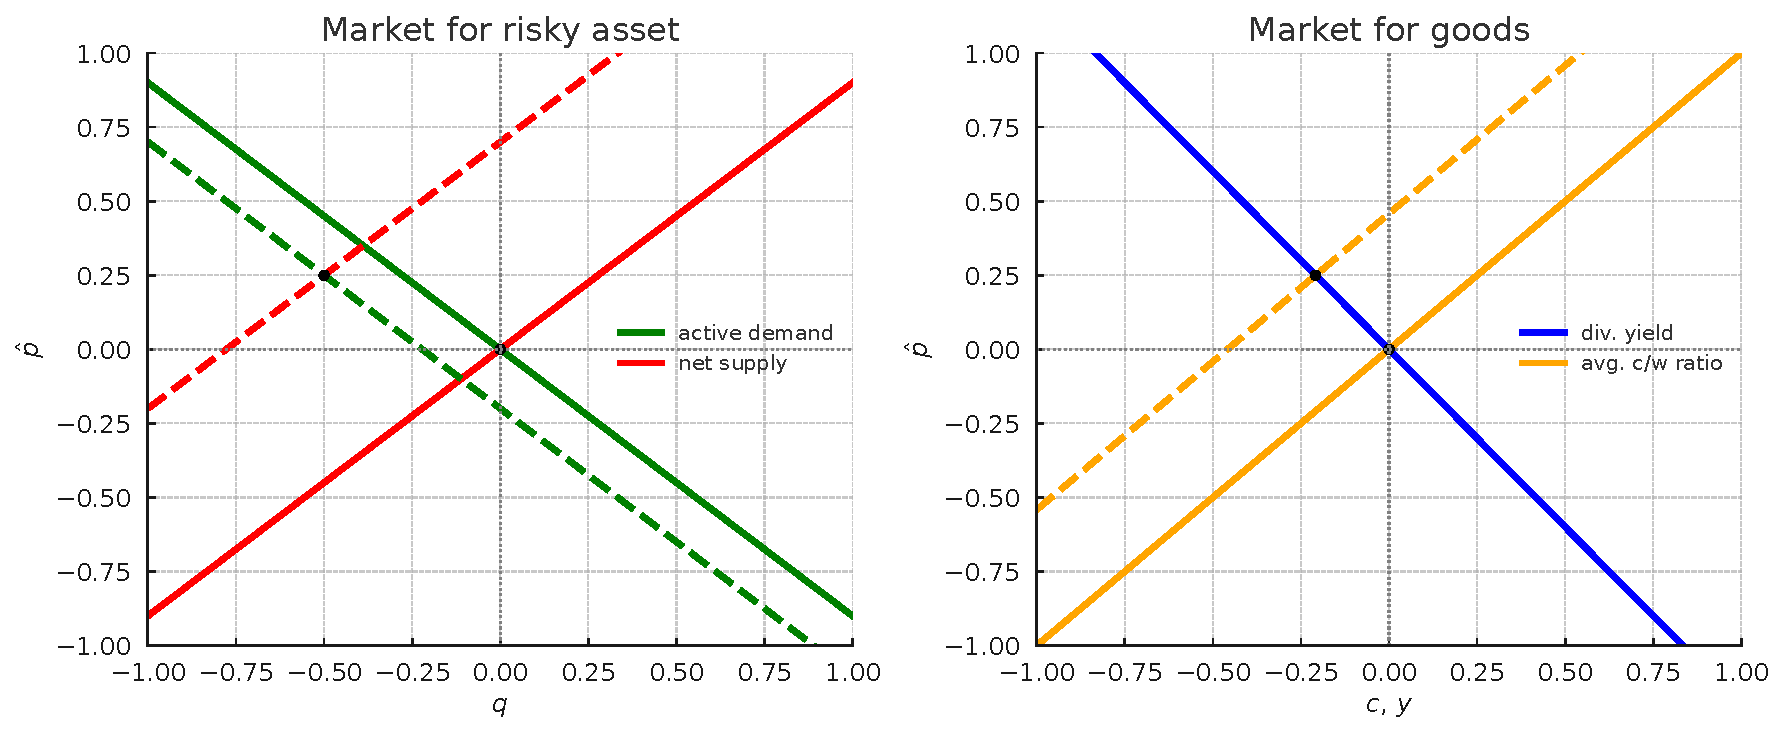
\includegraphics[width=0.95\linewidth]{figures/mkt_equilibrium2.pdf}
%     \caption{Equilibrium with inefficient risk allocation: risky-asset (left) and goods (right) markets.}
%     \label{fig:mkt_equilibrium2}
% \end{figure}


% Figure~\ref{fig:mkt_equilibrium2} illustrates the effects of portfolio flows when risk is initially concentrated on active investors, i.e., $\overline{\alpha}_{p,t}<1$. An inflow into the risky asset shifts the average consumption–wealth ratio curve leftward (right panel) and the net-supply curve leftward (left panel). The interest rate then adjusts so that active demand meets net supply at the goods-clearing price. In this case, portfolio flows have a positive price impact—the aggregate market elasticity is \emph{finite}.

% \begin{prop}[Aggregate elasticity: inefficient passive demand]\label{prop:elasticity_passive_demand}
%     % Suppose $\rho>\left(1-\psi^{-1}\right)\left( \mu - \frac{\gamma\|\sigma\|^2}{2}  \right)$. 
%     Without preference heterogeneity and leverage constraints, the inverse aggregate market elasticity $ \varepsilon^{-1}_{M,t} $ is
%     \begin{equation}\label{eq:elasticity_passive_demand}
%         \varepsilon_{M,t}^{-1}
%         \;=\;
%         -\,(\chi_{p}+y^*)^{-1}\,\frac{\partial \chi_{0,t}}{\partial f_t}
%         \;=\;
%         \left(1-\psi^{-1}\right)\frac{\gamma \|\sigma\|^{2}}{y^*}
%         \frac{1-\overline{\alpha}_{p,t}}{x_{a,t}}
%         \;+\;\mathcal{O}\!\left(\epsilon^{2}\right),
%     \end{equation}
%     where $x_{a,t}\equiv 1-x_{0,t}$ is the wealth share of active investors and $y^*\equiv 1/p^*$.
% \end{prop}

% Proposition~\ref{prop:elasticity_passive_demand} highlights the determinants of aggregate market elasticity. In contrast to \citet{gabaix2020search}, the risky-asset price elasticity $\zeta_p$—and the cross-elasticity $\zeta_r$—do not directly affect the aggregate elasticity. Given the recursive property of the demand system (where $r_t$ enters only the risky-asset demand), the price impact is determined by the properties of the consumption–wealth ratio.

% The market elasticity is finite whenever $\overline{\alpha}_{p,t}\neq 1$ and $\psi\neq 1$. In the unit-EIS case, the price–dividend ratio is pinned down by the subjective discount rate, so portfolio flows generate offsetting movements in the risk premium and the risk-free rate. When $\overline{\alpha}_{p,t}=1$, the risk allocation is initially efficient and, again, there is no price impact.

% The price impact is positive when $\psi>1$ and $\overline{\alpha}_{p,t}<1$: interest-rate adjustments no longer fully offset the response of the risk premium, so the risk-premium effect dominates. This parallels representative-agent models where uncertainty shocks require $\psi>1$ for the risk-premium channel to dominate \citep[e.g.,][]{bansal2004risks}.

% The state-global perturbation approach also shows that aggregate elasticity is \emph{state dependent}. 
% Figure~\ref{Fig:elasticity_passive-demand} plots the price impact as a function of active investors' wealth for different passive-share levels: it is larger when active investors are under-capitalized, highlighting the role of their risk-bearing capacity. 
% Price impact also increases with the distance of the passive share from its optimal value.
% For instance, when passive investors do not participate in equities ($\overline{\alpha}_{p,t}=0$), we recover a version of \citet{basak1998equilibrium} in which price impact is maximized.

% \begin{figure}[!t]
%     \centering
%     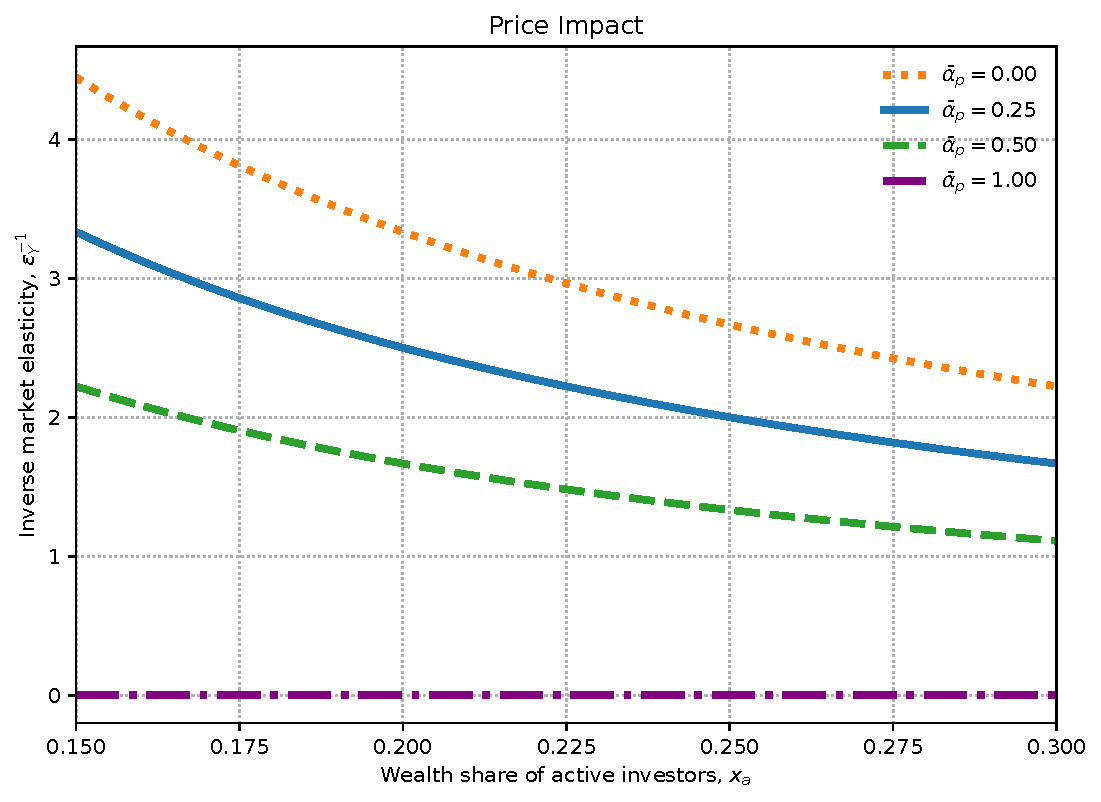
\includegraphics[width=0.65\textwidth]{./figures/price_impact_passive2.pdf}
%     \caption{Price impact: inefficient passive demand.}
%     \label{Fig:elasticity_passive-demand}
% \end{figure}

\subsection{Inefficient passive demand}

We next turn to a second-order approximation of the demand system to study how risk allocation affects aggregate market elasticity. To focus on the mechanism most clearly, consider the special case without preference heterogeneity or leverage constraints.  

\paragraph{The role of risk misallocation.}  
In this setting, demand for the risky asset is still given by \eqref{eq:demand_risky} up to second order. Without heterogeneity, the relevant demand shifter is  
\[
    f_t \equiv x_{0,t}\left(\overline{\alpha}_{p,t}-1\right),
\]
where $x_{0,t}$ denotes the wealth share of passive investors.  

The key difference relative to the benchmark arises from the consumption-wealth ratio. Aggregating \eqref{eq:xi_j} across investors, letting $c_t \equiv \sum_{j=0}^J x_{j,t} c_{j,t}$, and imposing market clearing $\sum_{j=0}^J x_{j,t}\alpha_{j,t}=1$, yields
\begin{equation}
    c_t
    \;=\;
    \psi\rho
    \;+\;
    (1-\psi)\!\left[
        r_t+\pi_t
        - \frac{\gamma\|\sigma\|^2}{2}\sum_{j=0}^J x_{j,t}\alpha_{j,t}^2
    \right]
    \;+\; \mathcal{O}(\epsilon^3).
\end{equation}
Under the efficient allocation $\alpha_{j,t}=1$, so $\sum_{j} x_{j,t}\alpha_{j,t}^2 = 1$. 
Any deviation from this efficient allocation creates dispersion in portfolios, leading to $\sum_j x_{j,t}\alpha_{j,t}^2>1$ by Jensen’s inequality, which lowers the risk-adjusted expected return $r_t+\pi_t - \tfrac{\gamma\|\sigma\|^2}{2}\sum_j x_{j,t}\alpha_{j,t}^2$. When $\psi>1$, this reduction weakens incentives to save and raises the consumption-wealth ratio for a given $r_t+\pi_t$.  

Movements in the passive portfolio therefore shift the aggregate consumption–wealth ratio. Its second-order expansion is
\begin{equation}
    \hat c_t \;\equiv\; c_t - c^*
    \;=\; \chi_{0,t} \;+\; \chi_p\,\hat p_t \;+\; \mathcal{O}(\epsilon^3),
\end{equation}
with coefficients
\[
    \chi_p = (\psi-1)\,\frac{1}{p^*},
    \qquad
    \chi_{0,t} = (\psi-1)\,\frac{\gamma\|\sigma\|^2}{2}\,
                    \frac{f_t^2}{x_{0,t}(1-x_{0,t})}.
\]
Because $\chi_{0,t}$ is quadratic in the flow $f_t$, it is $\mathcal{O}(\epsilon^2)$. For example, when passive investors are initially underexposed to the risky asset ($\overline{\alpha}_{p,t}<1$ and $\psi>1$), an inflow into stocks reduces the consumption-wealth ratio:
\[
    \frac{\partial \chi_{0,t}}{\partial f_t}
    \;=\;
    -\,(\psi-1)\,\gamma\|\sigma\|^2\,\frac{1-\overline{\alpha}_{p,t}}{1-x_{0,t}}.
\]
Note that $\chi_{0,t}$ is locally insensitive to portfolio flow changes when passive portfolio is efficient ($\overline{\alpha}_{p,t}=1$), consistent with the first-order analysis.  

\begin{figure}[t!]
    \centering
    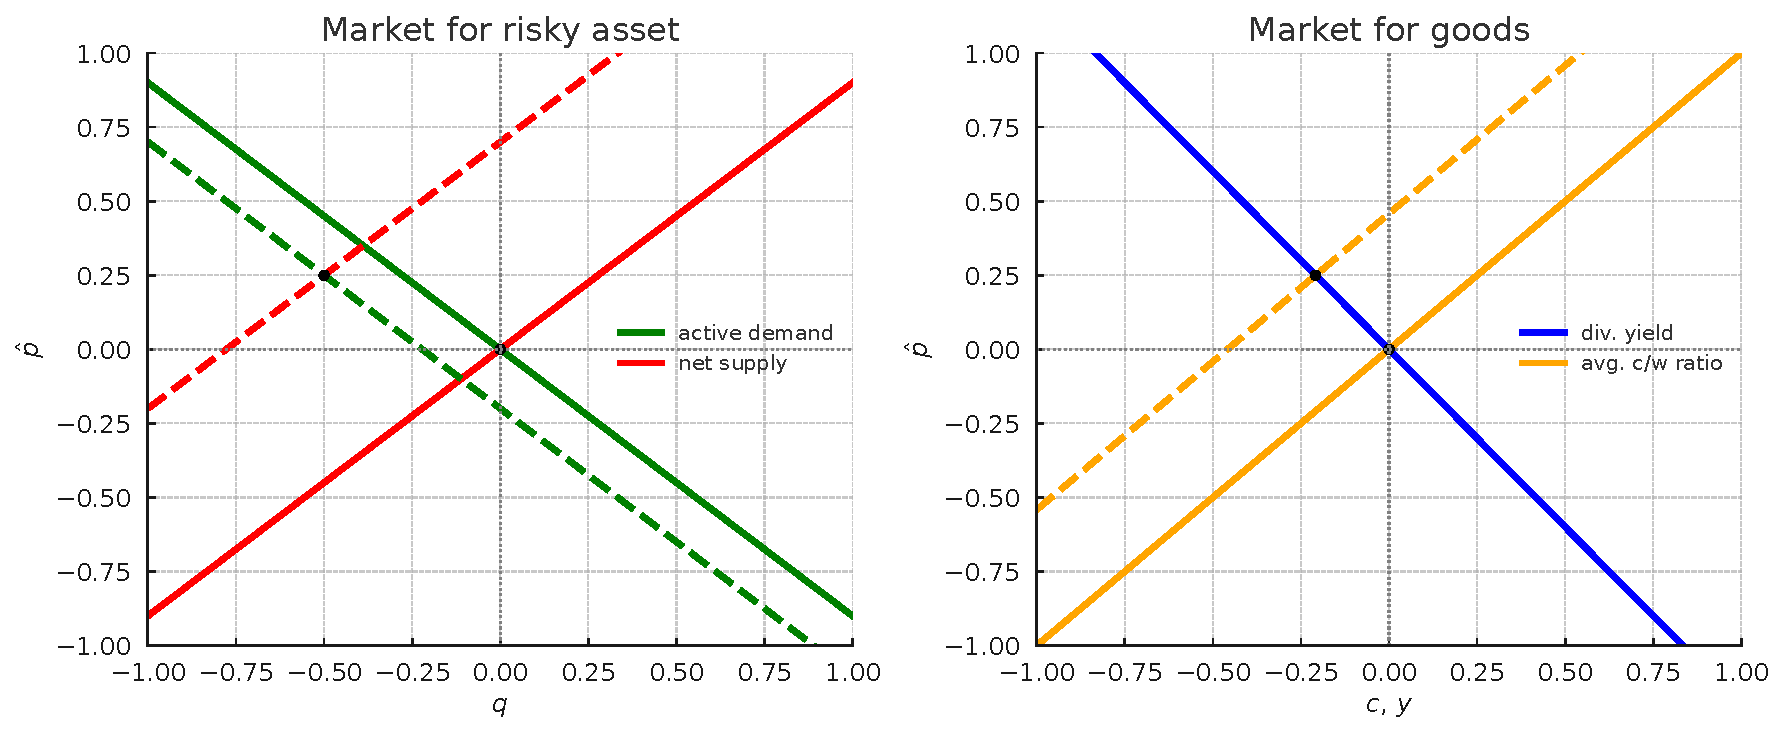
\includegraphics[width=0.95\linewidth]{figures/mkt_equilibrium2.pdf}
    \vspace{2mm}
    \caption{Equilibrium with inefficient risk allocation: risky asset (left) and goods (right) markets.}
    \label{fig:mkt_equilibrium2}
\end{figure}

Figure~\ref{fig:mkt_equilibrium2} illustrates the effects of portfolio flows when passive investors are initially underexposed to risk, i.e., $\overline{\alpha}_{p,t}<1$. An inflow into the risky asset shifts both the net supply curve (left panel) and the average consumption-wealth ratio schedule (right panel) leftward. The interest rate adjusts so that active demand meets net supply at the goods market clearing price. In this case, portfolio flows have a positive price impact and the aggregate elasticity is \textit{finite}.  

\begin{prop}[Aggregate elasticity: inefficient passive demand]\label{prop:elasticity_passive_demand}
Without preference heterogeneity or leverage constraints, the inverse aggregate elasticity is
\begin{equation}\label{eq:elasticity_passive_demand}
    \varepsilon_{M,t}^{-1}
    \;=\;
    -\,(\chi_{p}+y^*)^{-1}\,\frac{\partial \chi_{0,t}}{\partial f_t}
    \;=\;
    \left(1-\psi^{-1}\right)\frac{\gamma \|\sigma\|^{2}}{y^*}
    \frac{1-\overline{\alpha}_{p,t}}{x_{a,t}}
    \;+\;\mathcal{O}\!\left(\epsilon^{2}\right),
\end{equation}
where $x_{a,t}=1-x_{0,t}$ is the wealth share of active investors and $y^*=1/p^*$ is the dividend-price ratio in the benchmark economy.
\end{prop}

Proposition~\ref{prop:elasticity_passive_demand} shows that, unlike in \citet{gabaix2020search}, the risky-asset elasticities $\zeta_p$ and $\zeta_r$ are not the direct drivers of aggregate elasticity. Because the demand system is recursive (interest rates only enters the risky asset demand) the overall price impact is governed instead by how portfolio flows impact the consumption-wealth ratio. %In other words, aggregate elasticity reflects changes in savings behavior rather than the direct slope of risky asset demand.


The macro elasticity is finite whenever $\overline{\alpha}_{p,t}\neq 1$ and $\psi\neq 1$. In the unit EIS case, the price-dividend ratio is pinned down by the subjective discount rate, so portfolio flows generate offsetting movements in the risk premium and the risk-free rate. With efficient risk allocation ($\overline{\alpha}_{p,t}=1$), there is again no price impact.  

The price impact is positive when $\psi>1$ and $\overline{\alpha}_{p,t}<1$: interest rate adjustments no longer fully offset the risk premium response, so the latter dominates. This mirrors representative agent models in which uncertainty shocks affect prices only when $\psi>1$ \citep[e.g.,][]{bansal2004risks}.  

The state-global perturbation analysis also makes clear that elasticity is state dependent. Figure~\ref{Fig:elasticity_passive-demand} plots the price impact as a function of active investors' wealth for different passive-share levels.  Price impact rises when active investors are under capitalized, reflecting their limited risk-bearing capacity, and when the passive share deviates further from its efficient level. In the extreme case where passive investors hold no equities ($\overline{\alpha}_{p,t}=0$), we recover a version of \citet{basak1998equilibrium} in which price impact is maximized.  


\begin{figure}[!t]
    \centering
    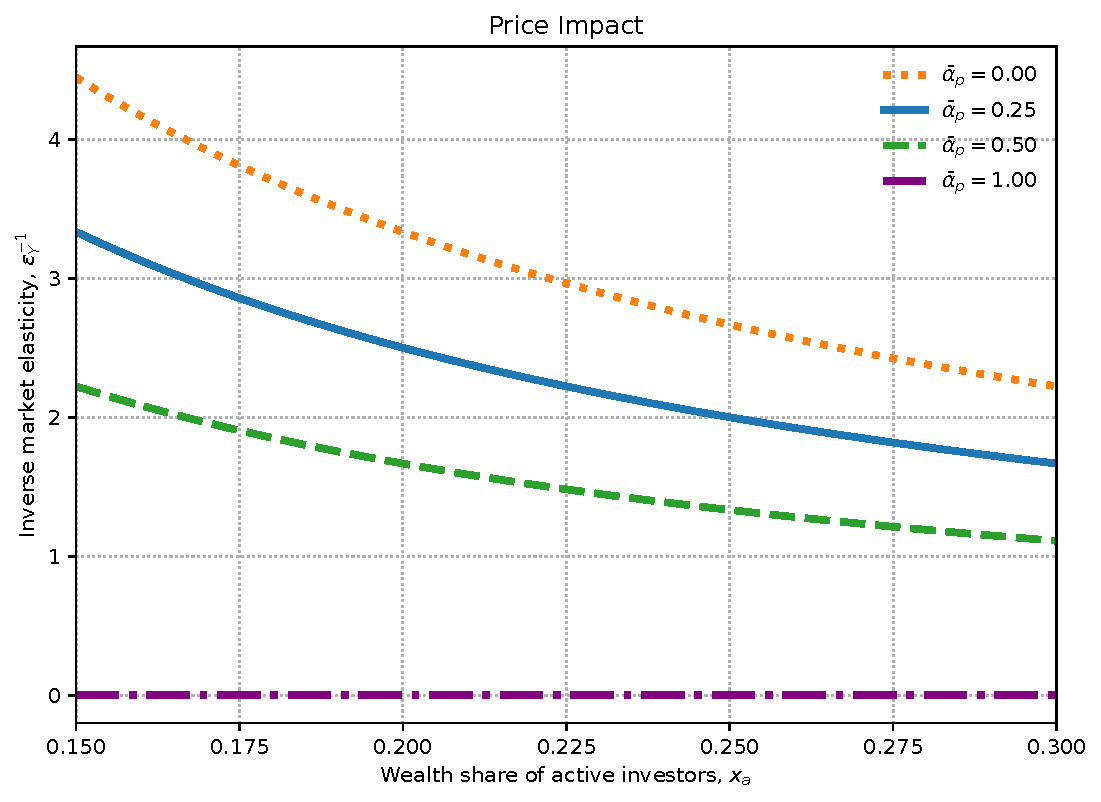
\includegraphics[width=0.65\textwidth]{./figures/price_impact_passive2.pdf}
    \vspace{2mm}
    \caption{Price impact: inefficient passive demand.}
    \label{Fig:elasticity_passive-demand}
\end{figure}



% In the absence of heterogeneity and leverage constraints, the demand for the risky asset under a second-order approximation takes the form in Equation \eqref{eq:demand_risky}, as shown in the appendix. In contrast, the consumption-wealth ratio is now given by
% \begin{equation}
%     c_{j,t} = \psi \rho + (1-\psi) \left[ r_t + \pi_t \alpha_{j,t} - \frac{\gamma \sigma^2}{2} \alpha_{j,t}^2 \right] + \xi_{j,t} + \mathcal{O}(\epsilon^3),
% \end{equation}
% where $\alpha_{0,t} = \overline{\alpha}_p $ and $\alpha_{j,t} = \frac{1-x_{0,t} \overline{\alpha}_p}{1-x_{0,t}}$ for $j = 1,\ldots, J$. Aggregating across investors, and using the market clearing condition $\sum_{j=0}^J x_j \alpha_{j,t} = 1$, we obtain
% \begin{equation}
%     c_t = \psi \rho + (1-\psi) \left[ r_t + \pi_t - \frac{\gamma \sigma^2}{2} \sum_{j=0}^J x_j \alpha_{j,t}^2 \right] + \mathcal{O}(\epsilon^3).
% \end{equation}

% The average consumption-wealth ratio now depends on the distribution of the risky asset in the economy. 
% Under the optimal allocation, the portfolio share is equal to one, $\alpha_{j,t} =1 $, for all investors, so $\sum_{j=0}^J x_j \alpha_{j,t}^2 = 1$. Any deviation of the optimal allocation creates dispersion in portfolios, so 
% $\sum_{j=0}^J x_j \alpha_{j,t}^2 > 1$, which reduces the risk-adjusted expected return $r_t + \pi_t - \frac{\gamma \sigma^2}{2} \sum_{j=0}^J x_j \alpha_{j,t}^2$. 
% If $\psi > 1$, the reduction in risk-adjusted returns weakens investors incentive to save, for any given level of $r_t +\pi_t$. 
% Therefore, the consumption-wealth ratio depends on how risk is allocated in the economy. 



% \begin{figure}[t!]
%     \centering

% \tikzset{every picture/.style={line width=0.75pt}} %set default line width to 0.75pt        

% \begin{tikzpicture}[x=0.75pt,y=0.75pt,yscale=-1,xscale=1]
% %uncomment if require: \path (0,235); %set diagram left start at 0, and has height of 235

% %Shape: Axis 2D [id:dp8667675453427319] 
% \draw [color={rgb, 255:red, 0; green, 0; blue, 0 }  ,draw opacity=1 ][line width=1.5]  (50,200) -- (289,200)(70,39) -- (70,222) (282,195) -- (289,200) -- (282,205) (65,46) -- (70,39) -- (75,46) (101,195) -- (101,205)(132,195) -- (132,205)(163,195) -- (163,205)(194,195) -- (194,205)(225,195) -- (225,205)(256,195) -- (256,205)(65,169) -- (75,169)(65,138) -- (75,138)(65,107) -- (75,107)(65,76) -- (75,76) ;
% \draw   ;
% %Shape: Arc [id:dp531658316023164] 
% \draw  [draw opacity=0][line width=2.25]  (69.96,200.56) .. controls (71.64,129.28) and (117.82,72.55) .. (173.1,73.85) .. controls (226.88,75.12) and (269.47,130.84) .. (270.19,199.49) -- (170.06,202.92) -- cycle ; \draw  [color={rgb, 255:red, 208; green, 2; blue, 27 }  ,draw opacity=1 ][line width=2.25]  (69.96,200.56) .. controls (71.64,129.28) and (117.82,72.55) .. (173.1,73.85) .. controls (226.88,75.12) and (269.47,130.84) .. (270.19,199.49) ;  
% %Shape: Circle [id:dp05697314227899386] 
% \draw  [draw opacity=0][fill={rgb, 255:red, 248; green, 231; blue, 28 }  ,fill opacity=0.5 ] (141.33,77.67) .. controls (141.33,74.17) and (144.17,71.33) .. (147.67,71.33) .. controls (151.16,71.33) and (154,74.17) .. (154,77.67) .. controls (154,81.16) and (151.16,84) .. (147.67,84) .. controls (144.17,84) and (141.33,81.16) .. (141.33,77.67) -- cycle ;
% %Shape: Circle [id:dp7553623057031522] 
% \draw  [draw opacity=0][fill={rgb, 255:red, 139; green, 87; blue, 42 }  ,fill opacity=0.5 ] (187.33,77.67) .. controls (187.33,74.17) and (190.17,71.33) .. (193.67,71.33) .. controls (197.16,71.33) and (200,74.17) .. (200,77.67) .. controls (200,81.16) and (197.16,84) .. (193.67,84) .. controls (190.17,84) and (187.33,81.16) .. (187.33,77.67) -- cycle ;
% %Shape: Axis 2D [id:dp8452210536537006] 
% \draw [color={rgb, 255:red, 0; green, 0; blue, 0 }  ,draw opacity=1 ][line width=1.5]  (377,199) -- (616,199)(397,38) -- (397,221) (609,194) -- (616,199) -- (609,204) (392,45) -- (397,38) -- (402,45) (428,194) -- (428,204)(459,194) -- (459,204)(490,194) -- (490,204)(521,194) -- (521,204)(552,194) -- (552,204)(583,194) -- (583,204)(392,168) -- (402,168)(392,137) -- (402,137)(392,106) -- (402,106)(392,75) -- (402,75) ;
% \draw   ;
% %Straight Lines [id:da8694501852937826] 
% \draw [color={rgb, 255:red, 245; green, 166; blue, 35 }  ,draw opacity=1 ][line width=1.5]    (347,55) -- (631,217) ;
% %Straight Lines [id:da4872089001830353] 
% \draw [color={rgb, 255:red, 74; green, 144; blue, 226 }  ,draw opacity=1 ][line width=1.5]    (343,199) -- (603,50) ;
% %Shape: Circle [id:dp6153612433225819] 
% \draw  [draw opacity=0][fill={rgb, 255:red, 139; green, 87; blue, 42 }  ,fill opacity=1 ] (222.33,97.67) .. controls (222.33,94.17) and (225.17,91.33) .. (228.67,91.33) .. controls (232.16,91.33) and (235,94.17) .. (235,97.67) .. controls (235,101.16) and (232.16,104) .. (228.67,104) .. controls (225.17,104) and (222.33,101.16) .. (222.33,97.67) -- cycle ;
% %Shape: Circle [id:dp4728310817061825] 
% \draw  [draw opacity=0][fill={rgb, 255:red, 248; green, 231; blue, 28 }  ,fill opacity=1 ] (107.33,97.67) .. controls (107.33,94.17) and (110.17,91.33) .. (113.67,91.33) .. controls (117.16,91.33) and (120,94.17) .. (120,97.67) .. controls (120,101.16) and (117.16,104) .. (113.67,104) .. controls (110.17,104) and (107.33,101.16) .. (107.33,97.67) -- cycle ;
% %Straight Lines [id:da6317730272289139] 
% \draw [color={rgb, 255:red, 0; green, 0; blue, 0 }  ,draw opacity=0.5 ][fill={rgb, 255:red, 0; green, 0; blue, 0 }  ,fill opacity=0 ]   (194,77.67) -- (226.93,96.67) ;
% \draw [shift={(228.67,97.67)}, rotate = 209.98] [color={rgb, 255:red, 0; green, 0; blue, 0 }  ,draw opacity=0.5 ][line width=0.75]    (10.93,-3.29) .. controls (6.95,-1.4) and (3.31,-0.3) .. (0,0) .. controls (3.31,0.3) and (6.95,1.4) .. (10.93,3.29)   ;
% %Straight Lines [id:da22117887446043505] 
% \draw [color={rgb, 255:red, 0; green, 0; blue, 0 }  ,draw opacity=0.5 ][fill={rgb, 255:red, 0; green, 0; blue, 0 }  ,fill opacity=0 ]   (147.67,77.67) -- (115.39,96.65) ;
% \draw [shift={(113.67,97.67)}, rotate = 329.53] [color={rgb, 255:red, 0; green, 0; blue, 0 }  ,draw opacity=0.5 ][line width=0.75]    (10.93,-3.29) .. controls (6.95,-1.4) and (3.31,-0.3) .. (0,0) .. controls (3.31,0.3) and (6.95,1.4) .. (10.93,3.29)   ;
% %Straight Lines [id:da6847983852102553] 
% \draw [color={rgb, 255:red, 74; green, 144; blue, 226 }  ,draw opacity=1 ][line width=1.5]  [dash pattern={on 1.69pt off 2.76pt}]  (348,206) -- (608,57) ;

% % Text Node
% \draw (284,214) node  [color={rgb, 255:red, 0; green, 0; blue, 0 }  ,opacity=1 ,rotate=-358.98]  {$port.\ share$};
% % Text Node
% \draw (42,39) node  [color={rgb, 255:red, 0; green, 0; blue, 0 }  ,opacity=1 ,rotate=-358.98]  {$return$};
% % Text Node
% \draw (74,10.43) node [anchor=north west][inner sep=0.75pt]   [align=left] {\textbf{Risk-adjusted excess return}};
% % Text Node
% \draw (544,67) node  [color={rgb, 255:red, 74; green, 144; blue, 226 }  ,opacity=1 ,rotate=-329.57]  {$avg.\ c/w\ ratio$};
% % Text Node
% \draw (639,200) node  [color={rgb, 255:red, 0; green, 0; blue, 0 }  ,opacity=1 ,rotate=-358.98]  {$c,y$};
% % Text Node
% \draw (578,170) node  [color={rgb, 255:red, 245; green, 166; blue, 35 }  ,opacity=1 ,rotate=-28.61]  {$div.\ yield$};
% % Text Node
% \draw (381,38) node  [color={rgb, 255:red, 0; green, 0; blue, 0 }  ,opacity=1 ,rotate=-358.98]  {$p$};
% % Text Node
% \draw (434,3.43) node [anchor=north west][inner sep=0.75pt]   [align=left] {\textbf{Market for goods}};
% % Text Node
% \draw (239,89) node [anchor=north west][inner sep=0.75pt]   [align=left] {\textbf{a}};
% % Text Node
% \draw (95,87) node [anchor=north west][inner sep=0.75pt]   [align=left] {\textbf{p}};


% \end{tikzpicture}    
% \caption{Consumption-wealth ratio when risk is nearly perfectly allocated}    \label{fig:mkt_equilibrium_misallocation}
% \end{figure}

% Figure~\ref{fig:mkt_equilibrium_misallocation2} illustrates how an increase in risk misallocation affects the equilibrium in the goods market. 
% The left panel represents the risk-adjusted excess return, $\pi_t \alpha_{j,t} - \frac{\gamma \sigma^2}{2} \alpha_{j,t}^2$, as a function of the portfolio share $\alpha_{j,t}$. 
% Suppose that the passive investor has initially a portfolio share that is less than one and then decides to further reduce its holding of the risky asset, as represented by the yellow dot in the figure. 
% Even if the risk premium is constant, the risk-adjusted return is reduced, as the investor moves  away from the optimal holding of the risky asset. 
% The portfolio share of the active investors also moves away from the optimal, as represented by the brown dot in the figure, so the risk-adjusted return is reduced for them as well. 
% Therefore, both agents have a weaker incentive to save, which leads to a shift in the average consumption-wealth ratio, as shown in the right panel. 

% \begin{figure}[t!]
%     \centering

%     \begin{tikzpicture}[x=0.75pt,y=0.75pt,yscale=-1,xscale=1]
% %uncomment if require: \path (0,235); %set diagram left start at 0, and has height of 235

% %Shape: Axis 2D [id:dp17811910341215076] 
% \draw [color={rgb, 255:red, 0; green, 0; blue, 0 }  ,draw opacity=1 ][line width=1.5]  (50,200) -- (289,200)(70,39) -- (70,222) (282,195) -- (289,200) -- (282,205) (65,46) -- (70,39) -- (75,46) (101,195) -- (101,205)(132,195) -- (132,205)(163,195) -- (163,205)(194,195) -- (194,205)(225,195) -- (225,205)(256,195) -- (256,205)(65,169) -- (75,169)(65,138) -- (75,138)(65,107) -- (75,107)(65,76) -- (75,76) ;
% \draw   ;
% %Shape: Arc [id:dp2728896334946356] 
% \draw  [draw opacity=0][line width=2.25]  (69.96,200.56) .. controls (71.64,129.28) and (117.82,72.55) .. (173.1,73.85) .. controls (226.88,75.12) and (269.47,130.84) .. (270.19,199.49) -- (170.06,202.92) -- cycle ; \draw  [color={rgb, 255:red, 208; green, 2; blue, 27 }  ,draw opacity=1 ][line width=2.25]  (69.96,200.56) .. controls (71.64,129.28) and (117.82,72.55) .. (173.1,73.85) .. controls (226.88,75.12) and (269.47,130.84) .. (270.19,199.49) ;  
% %Shape: Circle [id:dp09152732788574003] 
% \draw  [draw opacity=0][fill={rgb, 255:red, 248; green, 231; blue, 28 }  ,fill opacity=0.5 ] (105.33,100.67) .. controls (105.33,97.17) and (108.17,94.33) .. (111.67,94.33) .. controls (115.16,94.33) and (118,97.17) .. (118,100.67) .. controls (118,104.16) and (115.16,107) .. (111.67,107) .. controls (108.17,107) and (105.33,104.16) .. (105.33,100.67) -- cycle ;
% %Shape: Circle [id:dp8702384042700901] 
% \draw  [draw opacity=0][fill={rgb, 255:red, 139; green, 87; blue, 42 }  ,fill opacity=0.5 ] (224.33,100.67) .. controls (224.33,97.17) and (227.17,94.33) .. (230.67,94.33) .. controls (234.16,94.33) and (237,97.17) .. (237,100.67) .. controls (237,104.16) and (234.16,107) .. (230.67,107) .. controls (227.17,107) and (224.33,104.16) .. (224.33,100.67) -- cycle ;
% %Shape: Axis 2D [id:dp6014255008545599] 
% \draw [color={rgb, 255:red, 0; green, 0; blue, 0 }  ,draw opacity=1 ][line width=1.5]  (377,199) -- (616,199)(397,38) -- (397,221) (609,194) -- (616,199) -- (609,204) (392,45) -- (397,38) -- (402,45) (428,194) -- (428,204)(459,194) -- (459,204)(490,194) -- (490,204)(521,194) -- (521,204)(552,194) -- (552,204)(583,194) -- (583,204)(392,168) -- (402,168)(392,137) -- (402,137)(392,106) -- (402,106)(392,75) -- (402,75) ;
% \draw   ;
% %Straight Lines [id:da943055555850097] 
% \draw [color={rgb, 255:red, 245; green, 166; blue, 35 }  ,draw opacity=1 ][line width=1.5]    (347,55) -- (631,217) ;
% %Straight Lines [id:da12202983705810633] 
% \draw [color={rgb, 255:red, 74; green, 144; blue, 226 }  ,draw opacity=1 ][line width=1.5]    (343,199) -- (603,50) ;
% %Shape: Circle [id:dp9185533411503766] 
% \draw  [draw opacity=0][fill={rgb, 255:red, 139; green, 87; blue, 42 }  ,fill opacity=1 ] (259.33,160.67) .. controls (259.33,157.17) and (262.17,154.33) .. (265.67,154.33) .. controls (269.16,154.33) and (272,157.17) .. (272,160.67) .. controls (272,164.16) and (269.16,167) .. (265.67,167) .. controls (262.17,167) and (259.33,164.16) .. (259.33,160.67) -- cycle ;
% %Shape: Circle [id:dp458319980377794] 
% \draw  [draw opacity=0][fill={rgb, 255:red, 248; green, 231; blue, 28 }  ,fill opacity=1 ] (71.33,159.67) .. controls (71.33,156.17) and (74.17,153.33) .. (77.67,153.33) .. controls (81.16,153.33) and (84,156.17) .. (84,159.67) .. controls (84,163.16) and (81.16,166) .. (77.67,166) .. controls (74.17,166) and (71.33,163.16) .. (71.33,159.67) -- cycle ;
% %Straight Lines [id:da5461592683560248] 
% \draw [color={rgb, 255:red, 0; green, 0; blue, 0 }  ,draw opacity=0.5 ][fill={rgb, 255:red, 0; green, 0; blue, 0 }  ,fill opacity=0 ]   (230.67,100.67) -- (264.66,158.94) ;
% \draw [shift={(265.67,160.67)}, rotate = 239.74] [color={rgb, 255:red, 0; green, 0; blue, 0 }  ,draw opacity=0.5 ][line width=0.75]    (10.93,-3.29) .. controls (6.95,-1.4) and (3.31,-0.3) .. (0,0) .. controls (3.31,0.3) and (6.95,1.4) .. (10.93,3.29)   ;
% %Straight Lines [id:da04864508639252052] 
% \draw [color={rgb, 255:red, 0; green, 0; blue, 0 }  ,draw opacity=0.5 ][fill={rgb, 255:red, 0; green, 0; blue, 0 }  ,fill opacity=0 ]   (111.67,100.67) -- (78.67,157.93) ;
% \draw [shift={(77.67,159.67)}, rotate = 299.95] [color={rgb, 255:red, 0; green, 0; blue, 0 }  ,draw opacity=0.5 ][line width=0.75]    (10.93,-3.29) .. controls (6.95,-1.4) and (3.31,-0.3) .. (0,0) .. controls (3.31,0.3) and (6.95,1.4) .. (10.93,3.29)   ;
% %Straight Lines [id:da7145890387073353] 
% \draw [color={rgb, 255:red, 74; green, 144; blue, 226 }  ,draw opacity=1 ][line width=1.5]  [dash pattern={on 1.69pt off 2.76pt}]  (372,232) -- (632,83) ;

% % Text Node
% \draw (284,214) node  [color={rgb, 255:red, 0; green, 0; blue, 0 }  ,opacity=1 ,rotate=-358.98]  {$port.\ share$};
% % Text Node
% \draw (42,39) node  [color={rgb, 255:red, 0; green, 0; blue, 0 }  ,opacity=1 ,rotate=-358.98]  {$return$};
% % Text Node
% \draw (74,10.43) node [anchor=north west][inner sep=0.75pt]   [align=left] {\textbf{Risk-adjusted excess return}};
% % Text Node
% \draw (544,67) node  [color={rgb, 255:red, 74; green, 144; blue, 226 }  ,opacity=1 ,rotate=-329.57]  {$avg.\ c/w\ ratio$};
% % Text Node
% \draw (639,200) node  [color={rgb, 255:red, 0; green, 0; blue, 0 }  ,opacity=1 ,rotate=-358.98]  {$c,y$};
% % Text Node
% \draw (578,170) node  [color={rgb, 255:red, 245; green, 166; blue, 35 }  ,opacity=1 ,rotate=-28.61]  {$div.\ yield$};
% % Text Node
% \draw (381,38) node  [color={rgb, 255:red, 0; green, 0; blue, 0 }  ,opacity=1 ,rotate=-358.98]  {$p$};
% % Text Node
% \draw (434,3.43) node [anchor=north west][inner sep=0.75pt]   [align=left] {\textbf{Market for goods}};
% % Text Node
% \draw (247,152) node [anchor=north west][inner sep=0.75pt]   [align=left] {\textbf{a}};
% % Text Node
% \draw (90,151) node [anchor=north west][inner sep=0.75pt]   [align=left] {\textbf{p}};


% \end{tikzpicture}
%          \caption{Consumption-wealth ratio when risk is highly misallocated}
%     \label{fig:mkt_equilibrium_misallocation2}
% \end{figure}

% The magnitude of the shift in the average consumption-wealth ratio depends on the initial distribution of risk. 
% This point can be seen more clearly by writing the average consumption-wealth in terms of deviations from its value in the benchmark economy:
% \begin{equation}
%     \hat{c}_{t} = \zeta_{p}^c \hat{p}_t + \zeta_{0}^c,
% \end{equation}
% where $\zeta_0^c = (\psi-1) \frac{\gamma \sigma^2}{2} \sum_{j=0}^J x_j (\alpha_{j,t}-1)^2$. Notice that $\zeta_0^c$ is a function of $\overline{\alpha}_p$ and the derivative of $\zeta_0^c$ with respect to $\overline{\alpha}_p$ is given by
% \begin{equation}
%     \left. \frac{\partial \zeta_0^c}{\partial \overline{\alpha}_p} \right|_{\overline{\alpha}_p = 1} =  \left.(\psi-1) \gamma \sigma^2 \sum_{j=0}^J x_j (\alpha_{j,t}-1) \frac{\partial \alpha_{j,t}}{\partial \overline{\alpha}_p}\right|_{\overline{\alpha}_p = 1} = 0.
% \end{equation}
% If the passive investor initially holds the optimal portfolio, then a small change in $\overline{\alpha}_p$ has no impact in the consumption-wealth ratio. 
% This corresponds to the frictionless benchmark, which is analogous to the result under the first-order approximation. 
% However, if the initial allocation of risk is not optimal, changes in $\overline{\alpha}_p$ affect the consumption-wealth ratio. 
% Moreover, the effect is stronger the further the initial allocation is from the optimal. 
% This point is illustrated in Figure~\ref{fig:mkt_equilibrium_misallocation2}.
% The initial allocation is now further away from the optimal relative to the case in Figure~\ref{fig:mkt_equilibrium_misallocation2}, which leads to a larger decline in the risk-adjusted returns, as shown in the left panel. 
% In this case, we see a larger shift in the average consumption-wealth curve in the right panel. 



% \paragraph{The market elasticity with inefficient passive demand.} The equilibrium value for asset prices takes the same shape as in the case of the first-order approximation:
% \begin{equation}
%     \hat{p}_t = - \frac{\zeta_0^c}{\zeta_p^c + \frac{1}{p^*} }, \qquad \qquad 
%     \hat{r}_t = \frac{f_t}{\zeta_r^q} + \frac{\zeta_p^q}{\zeta_r^q \left( \zeta_p^c + \frac{1}{p^*} \right)} \zeta_0^c.\nonumber
% \end{equation}
% As before, the price of the risky asset is independent of the (micro) price elasticity $\zeta_p^q$. However, while the shifter $\zeta_0^c$ was independent of $\overline{\alpha}_p$ under a first-order approximation, this is not the case now, as $\zeta_0^c$ is a function of $\overline{\alpha}_p$. The next proposition derives the aggregate market elasticity in this case.

% \begin{prop}[Aggregate elasticity: inefficient passive demand]\label{prop:elasticity_passive_demand2}
% 	Suppose $\rho>\left(1-\psi^{-1}\right)\left( \mu - \frac{\gamma\sigma^2}{2}  \right)$. 
% 	If there is no preference heterogeneity and active investors do not face leverage constraints, the inverse aggregate market elasticity, $ 1/\varepsilon_M $, is given by:
% 	\begin{equation}\label{eq:elasticity_passive_demand}
% %		\frac{1}{p(X, \epsilon)} \frac{\partial p(X, \epsilon)}{\partial F(X, \epsilon)}
% 		\varepsilon_M^{-1}=\left(1-\psi^{-1}\right) \frac{\gamma \sigma^{2}}{y_{0}(X)} \frac{1-\overline{\alpha}_{p}}{x_{a}}+\mathcal{O}\left(\epsilon^{2}\right),		
% 	\end{equation}		
% 	where $ x_{a} \equiv 1-x_{0} $ denotes the wealth share of active investors and $y_0(x) = 1/p_0(X)$.
% \end{prop}
% \begin{proof}
% 	See Appendix~\ref{app:prop_elasticity_passive_demand}.
% \end{proof}



% We highlight several points from Proposition~\ref{prop:elasticity_passive_demand}. First, the price impact is equal to zero if $\overline{\alpha}_p$, that is, the market is infinitely elastic when risk is initially optimally allocated. Second, the price impact is also zero if the EIS is equal to one. 
% In this case, the consumption-wealth ratio is constant and $\zeta_0^c = 0$, so $\overline{\alpha}_p$ does not affect investors' incentive to save.
% Third, the market elasticity is positive if $\psi > 1$ and $\overline{\alpha}_p < 1$, so passive investors hold an inefficiently low share of the risky asset. 
% This result is consistent with the discussion in Section~\ref{sec:simple}, which shows that we obtain a finite elasticity when movements in the passive portfolio share shifts not only the net supply of risk to active investors, but also the consumption-wealth ratio. 
% As discussed above, risk misallocation provides a mechanism linking changes in $\overline{\alpha}_p$ to shifts in the consumption-wealth ratio. 
% % Moreover, the price impact is increasing in the degree of misallocation, as an increase in $\overline{\alpha}_p$ raises the price of the risky asset by more when $\overline{\alpha}_p$ is further away from 1, the optimal portfolio share in this economy. 
% Moreover, everything else constant, the price impact is largest in the case of no market participation by passive investors $(\overline{\alpha}_{p,t} = 0)$, as in e.g. \citet{basak1998equilibrium}, given that this corresponds to the maximum level of misallocation (given $\overline{\alpha}_p\geq 0$).
% Fourth, the elasticity is state-dependent and the price impact is larger when active investors are under-capitalized, that is, they hold a relatively small share of wealth. 
% Figure~\ref{Fig:elasticity_passive-demand} illustrate these points. We can see that the price impact is equal to zero when $\overline{\alpha}_p = 1$, it is positive when $\overline{\alpha}_p < 1$, it is decreasing in wealth share of active investors $x_a$, and it is largest when $\overline{\alpha}_p = 0$ for any given level of $x_a$.


% In Proposition~\ref{prop:second_order} in Appendix~\ref{app:prop_second_order}, we consider the second-order correction.
%\begin{prop}[Second-order correction]\label{prop:second_order}
%	Suppose $\rho>\left(1-\psi^{-1}\right)\left( \mu - \frac{\gamma
%		\sigma^2}{2}  \right)$.  Then,
%	\begin{enumerate}[(i)]
%		\item The second-order correction for the consumption-wealth ratio and risk exposure are given by:
%		\begin{align}
%		\xi_{j,2}(X) &= (1-\psi) \frac{\gamma \sigma^2}{2} \left[ \left(1-\psi^{-1}\right) \sum_{k=0}^J x_{k,t} \hat{\gamma}_k -\hat{\gamma}_j \right]\nonumber\\
%		%		\sigma_{j,1}(X) &= \sigma\min\left\{ \sum_{k\in\mathcal{J}^u} \frac{x_k}{x_u} \hat{\gamma}_k- \hat{\gamma}_j  -\frac{\hat{\alpha}_p  x_0+\frac{\hat{\sigma}}{\sigma} x_c }{1-x_0-x_c},\frac{\hat{\sigma}}{\sigma}  \right\}.\nonumber
%		\sigma_{j,2}(X) &= \frac{\eta_2(X)}{\gamma} - \frac{\eta_1(X)}{\gamma}\hat{\gamma}_j + \frac{\eta_0(X)}{\gamma}\hat{\gamma}_j^2 - (1-\gamma^{-1})   \sigma_{y,2}(X),\nonumber
%		\end{align}
%		where 
%		\begin{equation*}
%		\sigma_{y,2}(X)  = \left(1-\psi^{-1}\right)\frac{\gamma\sigma^2}{2 y_{0}(X)} \sum_{k=1}^J \left( \hat{\gamma}_k - \hat{\gamma}_0  \right) x_k \sigma_{k,1}(X).
%		\end{equation*}
%		\item The second-order correction for the Sharpe ratio, interest rate, and dividend yield are given by:
%		\begin{align}		
%		\eta_2(X) &=  - \frac{(\gamma-1) x_c + 1-x_0}{1-x_0-x_c} \sigma_{y,2}(X) - \gamma \sigma \mathbb{E}^u[\hat{\gamma}_j] \frac{ \hat{\alpha}_p x_0+ \frac{\hat{\sigma}}{\sigma}x_c }{1-x_0-x_c} - \gamma \sigma \var^u[\hat{\gamma}_j]\nonumber	\\	
%		%		r_1(X) &=\gamma\sigma^2 \left[ -\sum_{j\in\mathcal{J}^u} \frac{x_j}{x_u} \hat{\gamma}_j +\left(1-\psi^{-1}\right) \sum_{j=0}^J x_{j,t}\frac{\hat{\gamma}_j}{2}+\frac{\hat{\alpha}_p  x_0+\frac{\hat{\sigma}}{\sigma} x_c }{1-x_0-x_c} \right]\nonumber\\
%		r_2(X) &= - \eta_2(X) \sigma + \eta_0(X) \sigma_{y,2}(X)-\psi^{-1} (\mu_{y,2}(X) + \sigma \sigma_{y,2}(X))\nonumber\\
%		&\quad+ \left(1-\psi^{-1}\right) \sum_{j=0}^J x_{j} \gamma\sigma \left[ \sigma_{j,2}(X) + \frac{\sigma_{j,1}^2(X)}{2 \sigma} + \hat{\gamma}_j \sigma_{j,1} \right]\nonumber\\
%		&\quad+\psi^{-1} \sum_{j=0}^J x_{j}\left[ \mu_{\xi_j,2}(X) + (1-\gamma) \sigma_{\xi_j,2}(X) \sigma \right]\nonumber\\
%		y_2(X) &= \left(1-\psi^{-1}\right)\left[\gamma \sigma_{y, 2}(X) \sigma+\sum_{j=0}^{J} x_{j} \gamma \sigma\left(\frac{\sigma_{j, 1}^{2}(X)}{2 \sigma}+\sigma_{j, 2}(X)+\hat{\gamma}_{j} \sigma_{j, 1}(X)\right)\right],\nonumber
%		\end{align}
%		where 
%		\[\mathbb{E}^{u}[\hat{\gamma}_{j}] \equiv \sum_{j \in \mathcal{J}^{u}} \frac{x_{j}}{x_{u}} \hat{\gamma}_{j}, \quad \text { and } \quad \var^{u}[\hat{\gamma}_{j}] \equiv \sum_{j \in \mathcal{J}^{u}} \frac{x_{j}}{x_{u}} \hat{\gamma}_{j}^{2}-\left(\sum_{j \in \mathcal{J}^{u}} \frac{x_{j}}{x_{u}} \hat{\gamma}_{j}\right)^{2}.\]
%	\end{enumerate}
%\end{prop}
%\begin{proof}
%	See Appendix~\ref{app:prop_second_order}. 
%\end{proof}
%\textcolor{red}{Need to discuss the intuition and why we need to have second-order correction. Perhaps this needs to be moved after we discuss that there is no price impact up to first order.}
% We can write the second-order expansion of the price-dividend ratio $p(X,\epsilon)$ as:
% \begin{equation}
% p(X,\epsilon) = \frac{1}{y_0(X)} - \frac{y_1(X)}{y_0^2(X)} \epsilon + \left[ \frac{y_1^2(X)}{y_0^3(X)} - \frac{y_{2}(X)}{y_0^2(X)} \right] \epsilon^2 + \mathcal{O}(\epsilon^3).
% \end{equation}

% Therefore, we can derive the inverse elasticity as:
% \begin{equation}\label{eq:elasticity-y2}
% \varepsilon_M^{-1}=\frac{1}{p(X,\epsilon)}\frac{\partial p(X,\epsilon)}{\partial F(X,\epsilon)} = - \frac{1}{y_0(X)} \frac{\partial y_2(X)}{\partial \hat{\alpha}_p}\frac{\epsilon}{x_0} + \mathcal{O}(\epsilon^2),
% \end{equation}
% where the second-order correction of the dividend yield $ y_2 $ is given in Proposition~\ref{prop:second_order}. 
% Note that from Proposition~\ref{prop:first_order}, $ y_1(X) $ does not depend on $ \hat{\alpha}_p $, leading to no price impact (infinite elasticity) up to the first-order.





% \subsection{Passive demand}
% In Proposition~\ref{prop:elasticity_passive_demand}, we consider the impact of passive demand on the aggregate elasticity by shutting down preference heterogeneity and portfolio constraints.
% \begin{prop}[Aggregate elasticity: passive demand]\label{prop:elasticity_passive_demand2}
% 	Suppose $\rho>\left(1-\psi^{-1}\right)\left( \mu - \frac{\gamma\sigma^2}{2}  \right)$. 
% 	If there is no preference heterogeneity and active investors do not face leverage constraints, the inverse aggregate market elasticity, $ 1/\varepsilon_M $, is given by:
% 	\begin{equation}\label{eq:elasticity_passive_demand}
% %		\frac{1}{p(X, \epsilon)} \frac{\partial p(X, \epsilon)}{\partial F(X, \epsilon)}
% 		\varepsilon_M^{-1}=\left(1-\psi^{-1}\right) \frac{\gamma \sigma^{2}}{y_{0}(X)} \frac{1-\overline{\alpha}_{p}}{x_{a}}+\mathcal{O}\left(\epsilon^{2}\right),		
% 	\end{equation}		
% 	where $ x_{a} \equiv 1-x_{0} $ denotes the wealth share of active investors.
% \end{prop}
% \begin{proof}
% 	See Appendix~\ref{app:prop_elasticity_passive_demand}.
% \end{proof}
% We highlight several points from Proposition~\ref{prop:elasticity_passive_demand}. 
% %\textcolor{red}{The first point probably needs to move.} First, given that in the absence of investor heterogeneity and leverage constraints the second-order correction for the Sharpe ratio is zero ($ \eta_2(X) =0$), the price impact of flows is entirely driven by its second-order impact on the risk-free rate, $ r_2(X) $. In particular, we have $ r_2(X)=y_2(X) $, and
% %\begin{align}
% %	\frac{\partial \pi(X,\epsilon)}{\partial F(X,\epsilon)} &= 	-\frac{\gamma \sigma^2}{x_u}  +\mathcal{O}(\epsilon^2),\label{eq:rp-passive-demand}\\
% %	\frac{\partial r(X,\epsilon)}{\partial F(X,\epsilon)} &= \frac{\gamma \sigma^2}{x_u} +\left(1-\psi^{-1}\right) \gamma \sigma^{2} \frac{1-\overline{\alpha}_{p}}{x_{a}}+\mathcal{O}(\epsilon^2)\label{eq:r-passive-demand},
% %\end{align}
% %where $ \pi_t $ is the risk premium on the risky asset defined above.
% First, the price impact is stronger the smaller the passive investors' portfolio share $ \overline{\alpha}_p $. This is shown in Figure~\ref{Fig:elasticity_passive-demand}. Consider the extreme case of no market participation by passive investors when $ \overline{\alpha}_p=0 $ (as in e.g., \citealp{basak1998equilibrium}). In this case, if we allow passive agents to permanently increase their risky asset holdings from 0 to $ W_0\hat{\alpha}_p\epsilon $, then with second-order correction, flows still have a price impact, leading to a finite market elasticity. %Again, with $ \psi>1 $, from Equation~\eqref{eq:elasticity_passive_demand}, we see an \textit{increase} in the price-dividend ratio as a result. 
% Notably, the market becomes more macro inelastic relative to the case in which there is passive demand and $ \overline{\alpha}_p>0 $. In other words, the more risk is concentrated in the hands of active investors, the more compensation they demand for holding the risky asset, and the more inelastic market becomes. %It's about quantity of risk reducing the misallocation of risk.
% %\textcolor{red}{Need to better explain the elasticity in the limited participation case.}

% \textbf{Compare with Koijen and Gabaix. How would we get a multiplier of 5 here?} 


% Second, with the second-order correction, if we start at the frictionless Lucas economy benchmark with $ \overline{\alpha}_p=1 $, we arrive at an infinite aggregate elasticity as before where flows have no impact on the price-dividend ratio. %This immediately follows from Equation~\eqref{eq:rp-passive-demand} and \eqref{eq:r-passive-demand}, as 
% In this case, the effect of portfolio flows on the risk premium and the risk-free rate exactly offset each other again.

% Next, the sign and magnitude of the aggregate market elasticity depends on the EIS, $ \psi $, reemphasizing the key role that GE effects play in our model. When passive investors sell bonds to invest in stocks, the risk premium and interest rate move in opposite directions. With $ \psi>1 $,  the risk premium goes down more, leading to an increase in the price-dividend ratio. 
% This is in contrast to Proposition~\ref{prop:elasticity_first_order} where these effects exactly cancel each other out leading to no price impact up to the first order.
% %\textcolor{red}{Perhaps also mention \cite{gabaix2020search} and their non-traditional GE/PE setting?}

% Finally, note that from Equation~\eqref{eq:elasticity_passive_demand}, the market elasticity is time-varying and state-dependent. In particular, as shown in Figure~\ref{Fig:elasticity_passive-demand}, when $ x_a $ is low and active investors are undercapitalized, there is a larger price response to flows and the market is more macro inelastic. 



% \subsection{Preference heterogeneity and leverage constraints}

% We now return to the model with preference heterogeneity and leverage constraints. 
% The next proposition provides the main result of this section.

% \begin{prop}[Aggregate elasticity: heterogeneity and leverage constraints]\label{prop_elasticity_pref_heterog}
%     The inverse aggregate market elasticity is
%     \begin{equation}\label{eq:elasticity_pref_heterog}
%         \varepsilon_{M,t}^{-1}
%         \;=\;
%         \bigl(1-\psi^{-1}\bigr)\,
%         \frac{\gamma\,\|\sigma\|^{2}}{y^*}\,
%         \frac{\overline{\alpha}_{p,t}^{\mathrm{opt}}-\overline{\alpha}_{p,t}}{x_{a,t}}\,
%         \bigl(1-x_{c,t}\bigr)
%         \;+\;\mathcal{O}\!\left(\epsilon^{2}\right),
%     \end{equation}
%     where \(x_{c,t}\) is the wealth share of \emph{constrained} active investors and the passive investors' optimal portfolio share is
%     \begin{equation}\label{eq:optimal_alpha_p}
%         \overline{\alpha}_{p,t}^{\mathrm{opt}}
%         \;=\;
%         1
%         \;-\;
%         \frac{x_{a,t}-x_{c,t}}{1-x_{c,t}}\,
%         \frac{\gamma_{0}-\mathbb{E}^{u}_{t}[\gamma_{j}]}{\gamma}
%         \;-\;
%         \frac{x_{c,t}}{1-x_{c,t}}
%         \Bigl(\frac{\overline{\sigma}}{\|\sigma\|}-1\Bigr),
%     \end{equation}
%     with \(x_{u,t}\equiv x_{a,t}-x_{c,t}\) the wealth share of \emph{unconstrained} actives and $\mathbb{E}^{u}_{t}[\gamma_{j}]
%         \;\equiv\;
%         \sum_{j\in\mathcal{J}^{u}}\frac{x_{j,t}}{x_{u,t}}\,\gamma_{j}.$
%     % \[
%         % \mathbb{E}^{u}_{t}[\gamma_{j}]
%         % \;\equiv\;
%         % \sum_{j\in\mathcal{J}^{u}}\frac{x_{j,t}}{x_{u,t}}\,\gamma_{j}.
%     % \]
% \end{prop}
\subsection{Preference heterogeneity and leverage constraints}

We now reintroduce preference heterogeneity and leverage constraints into the model. These features shift the conditions under which passive investors’ portfolios are efficient and therefore alter the aggregate market elasticity. The next proposition provides the main result.

\begin{prop}[Aggregate elasticity: heterogeneity and leverage constraints]\label{prop_elasticity_pref_heterog}
The inverse aggregate market elasticity is
\begin{equation}\label{eq:elasticity_pref_heterog}
    \varepsilon_{M,t}^{-1}
    \;=\;
    \bigl(1-\psi^{-1}\bigr)\,
    \frac{\gamma\,\|\sigma\|^{2}}{y^*}\,
    \frac{\overline{\alpha}_{p,t}^{\mathrm{opt}}-\overline{\alpha}_{p,t}}{x_{a,t}-x_{c,t}}\,
    \bigl(1-x_{c,t}\bigr)
    \;+\;\mathcal{O}\!\left(\epsilon^{2}\right),
\end{equation}
where $x_{c,t}$ is the wealth share of constrained active investors and the passive investors’ optimal portfolio share is
\begin{equation}\label{eq:optimal_alpha_p}
    \overline{\alpha}_{p,t}^{\mathrm{opt}}
    \;=\;
    1
    \;-\;
    \frac{x_{a,t}-x_{c,t}}{1-x_{c,t}}\,
    \frac{\gamma_{0}-\mathbb{E}^{u}_{t}[\gamma_{j}]}{\gamma}
    \;-\;
    \frac{x_{c,t}}{1-x_{c,t}}
    \Bigl(\frac{\overline{\sigma}}{\|\sigma\|}-1\Bigr),
\end{equation}
with $x_{u,t}\equiv x_{a,t}-x_{c,t}$ the wealth share of unconstrained active investors and 
\[
    \mathbb{E}^{u}_{t}[\gamma_{j}]
    \;\equiv\;
    \sum_{j\in\mathcal{J}^{u}}\frac{x_{j,t}}{x_{u,t}}\,\gamma_{j}.
\]
\end{prop}

% \begin{prop}[Aggregate elasticity: heterogeneity and leverage constraints]\label{prop_elasticity_pref_heterog}
% 	The inverse aggregate market elasticity, $ 1/\varepsilon_M $, is given by:
% 	\begin{equation}\label{eq:elasticity_pref_heterog}
% 	%\frac{1}{p(X, \epsilon)} \frac{\partial p(X, \epsilon)}{\partial F(X, \epsilon)}
% 	% \varepsilon_M^{-1}=\left(1-\psi^{-1}\right) \frac{\gamma \sigma^{2}}{y^*}\left[\frac{1-\overline{\alpha}_{p}}{x_{a}}-\frac{\gamma_{0}-\mathbb{E}^{u}[\gamma_{j}]}{\gamma}\right]+\mathcal{O}\left(\epsilon^{2}\right),
%     \varepsilon_{M,t}^{-1}=\left(1-\psi^{-1}\right) \frac{\gamma \sigma^{2}}{y^*}\frac{\overline{\alpha}_{p,t}^{optimal}-\overline{\alpha}_{p,t}}{x_{a,t}}(1-x_{c,t})+\mathcal{O}\left(\epsilon^{2}\right).
% 	\end{equation}
% 	where $x_{c,t}$ is the wealth share of constrained active investors, and the passive investor's optimal portfolio share is given by:
% 		\begin{equation}\label{eq:optimal_alpha_p}
%             \overline{\alpha}_{p,t}^{optimal} = 1 -\frac{x_{a,t} - x_{c,t}}{1-x_{c,t}}\frac{\gamma_0-\mathbb{E}_t^u[\gamma_j] }{\gamma} - \frac{x_{c,t}(\frac{\overline{\sigma}}{\|\sigma\|}-1)  }{1-x_{c,t}},
%         \end{equation}
%         and $\mathbb{E}_t^u[\gamma_j] \equiv \sum_{j\in\mathcal{J}^u} w_{j,t} \gamma_j,$ where $ w_{j,t} = \frac{x_{j,t}}{\sum_{j\in\mathcal{J}^u}} $ is the wealth share of type $j$ investor among unconstrained investors.
% \end{prop}
% \begin{proof}
% 	See Appendix~\ref{app:prop_elasticity_pref_heterog}.
% \end{proof}


% Proposition~\ref{prop_elasticity_pref_heterog} provides a complete characterization of the aggregate market elasticity in the full model. 
% As before, the market is infinitely elastic when passive investors hold their optimal portfolio share, \(\overline{\alpha}_{p,t}=\overline{\alpha}_{p,t}^{\mathrm{opt}}\). 
% With homogeneous preferences \(\bigl(\gamma_j = \gamma) \) and slack leverage constraints \(\bigl(x_{c,t} = 0\bigr)\), the optimal share reduces to \(1\). 
% More generally, preference heterogeneity and binding leverage constraints shift \(\overline{\alpha}_{p,t}^{\mathrm{opt}}\) away from unity as a function of the wealth distribution and risk aversion parameters.
Proposition~\ref{prop_elasticity_pref_heterog} characterizes aggregate market elasticity in the full model. As in the frictionless benchmark, the market remains infinitely elastic when passive investors hold their optimal portfolio share, $\overline{\alpha}_{p,t}=\overline{\alpha}_{p,t}^{\mathrm{opt}}$. 
The optimal portfolio share corresponds to the value of $\overline{\alpha}_{p,t}$ such that the passive investor would have no incentive to change their portfolio. 
Under homogeneous preferences ($\gamma_j=\gamma$) and slack leverage constraints ($x_{c,t}=0$), this condition reduces to $\overline{\alpha}_{p,t}=1$. More generally, preference heterogeneity and binding leverage constraints shift the efficient passive share away from unity, with its level determined by the wealth distribution and the relative risk aversion of different investor types.


% \paragraph{Preference heterogeneity.}
% To understand Proposition~\ref{prop_elasticity_pref_heterog}, first consider the case with slack leverage constraints, \(x_{c,t}=0\).
% Then \eqref{eq:optimal_alpha_p} simplifies to
% \[
% \overline{\alpha}_{p,t}^{\mathrm{opt}}
% = 1 - x_{a,t}\,\frac{\gamma_0-\mathbb{E}^u_t[\gamma_j]}{\gamma},
% \]
% so relative to the homogeneous case the only difference is that
% \(\overline{\alpha}_{p,t}^{\mathrm{opt}}\neq 1\) whenever \(\gamma_0\neq \mathbb{E}^u_t[\gamma_j]\).
% The price–impact expression \eqref{eq:elasticity_pref_heterog} becomes
% \[
% \varepsilon_{M,t}^{-1}
% = \bigl(1-\psi^{-1}\bigr)\,\frac{\gamma\|\sigma\|^2}{y^*}\,
% \frac{\overline{\alpha}_{p,t}^{\mathrm{opt}}-\overline{\alpha}_{p,t}}{x_{a,t}}
% \;+\;\mathcal{O}(\epsilon^2).
% \]

% Optimal risk sharing implies that if \(\gamma_0>\mathbb{E}^u_t[\gamma_j]\), that is passive investors are more risk averse than the active agents on average, then
% \(\partial \overline{\alpha}_{p,t}^{\mathrm{opt}}/\partial x_{a,t}= -(\gamma_0-\mathbb{E}^u_t[\gamma_j])/\gamma<0\):
% the passive investors’ \emph{optimal} equity share \emph{rises} as the active wealth share falls.
% This typically occurs after a negative aggregate shock, since active investors tend to be more exposed to risk.

% If passive investors do not rebalance after such a shock, market inelasticity increases for two reinforcing reasons:
% (i) the wealth share of actives \(x_{a,t}\) shrinks, reducing risk-bearing capacity; and
% (ii) the deviation \(\overline{\alpha}_{p,t}^{\mathrm{opt}}-\overline{\alpha}_{p,t}\) widens, moving the system farther from the optimal allocation.
% These forces produce a sharper rise in price impact as \(x_{a,t}\) declines, as illustrated in the left panel of Figure~\ref{fig:price_impact_comparison}, where the heterogeneous- and homogeneous-preference curves coincide at \(x_{a}=0.20\) but the former steepens markedly as \(x_a\) falls.
\paragraph{Preference heterogeneity.}
With slack leverage constraints ($x_{c,t}=0$), \eqref{eq:optimal_alpha_p} simplifies to
\[
\overline{\alpha}_{p,t}^{\mathrm{opt}}
= 1 - x_{a,t}\,\frac{\gamma_0-\mathbb{E}^u_t[\gamma_j]}{\gamma},
\]
so, unlike the homogeneous preference case, the efficient passive share $\overline{\alpha}_{p,t}^{\mathrm{opt}}$ differs from unity whenever $\gamma_0 \neq \mathbb{E}^u_t[\gamma_j]$. The inverse elasticity in \eqref{eq:elasticity_pref_heterog} becomes
\[
\varepsilon_{M,t}^{-1}
= \bigl(1-\psi^{-1}\bigr)\,\frac{\gamma\|\sigma\|^2}{y^*}\,
\frac{\overline{\alpha}_{p,t}^{\mathrm{opt}}-\overline{\alpha}_{p,t}}{x_{a,t}}
\;+\;\mathcal{O}(\epsilon^2).
\]

Optimal risk sharing implies that when passive investors are more risk averse than the average unconstrained active ($\gamma_0>\mathbb{E}^u_t[\gamma_j]$),
\[
\frac{\partial \overline{\alpha}_{p,t}^{\mathrm{opt}}}{\partial x_{a,t}}
= -\,\frac{\gamma_0-\mathbb{E}^u_t[\gamma_j]}{\gamma} < 0,
\]
so the efficient passive equity share rises as the active wealth share falls, typically after adverse aggregate shocks that erode active wealth that is more exposed to risk. If passive investors do not rebalance in such episodes, market inelasticity increases because $x_{a,t}$ declines (reducing risk-bearing capacity) while the gap $\overline{\alpha}_{p,t}^{\mathrm{opt}}-\overline{\alpha}_{p,t}$ widens (moving the economy farther from the efficient allocation). Consequently, price impact rises as $x_{a,t}$ falls, as shown in the left panel (a) of Figure~\ref{fig:price_impact_comparison}: the heterogeneous- and homogeneous-preference curves coincide at $x_{a}=0.20$, but only the former steepens markedly as $x_a$ declines.


\begin{figure}[t!]
    \centering
    % --- Left: homogeneous vs heterogeneous preferences ---
    \begin{subfigure}[t]{0.48\textwidth}
        \centering
        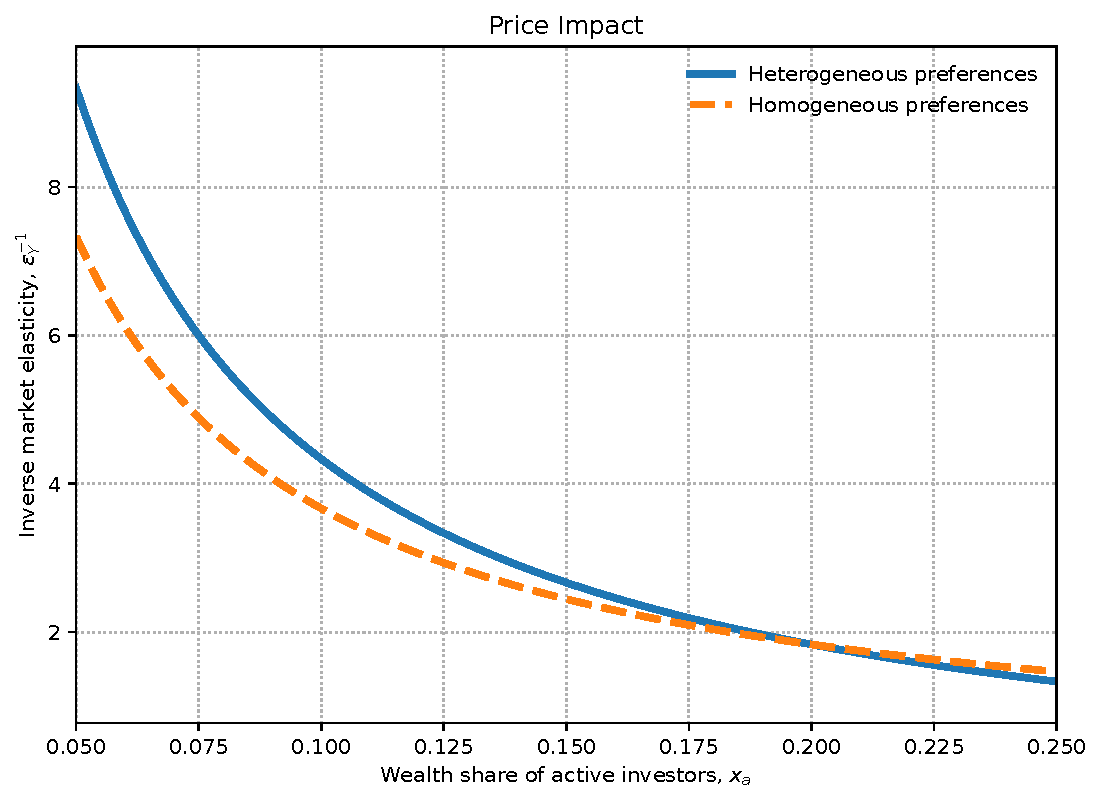
\includegraphics[width=\linewidth]{figures/price_impact_heterogeneity1.pdf}
        \caption{Homogeneous vs. heterogeneous preferences}
        \label{fig:impact_het_vs_hom}
    \end{subfigure}\hfill
    % --- Right: price impact vs w_1 for different \bar{\alpha}_p ---
    \begin{subfigure}[t]{0.48\textwidth}
        \centering
        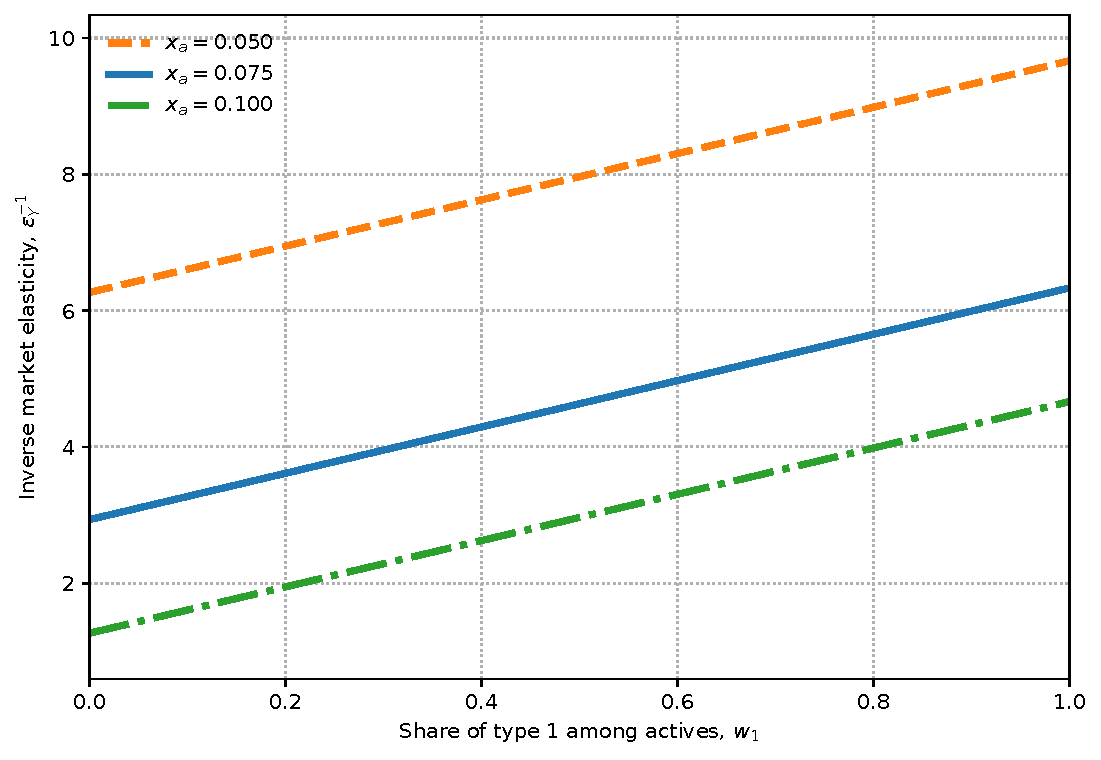
\includegraphics[width=\linewidth]{figures/price_impact_heterogeneity2.pdf}
        \caption{Role of wealth distribution of active investors}
        \label{fig:impact_vs_w1_by_alphap}
    \end{subfigure}
    \vspace{2mm}
    \caption{Price impact comparisons. Panel (a) compares heterogeneous and homogeneous preferences. Panel (b) shows the sensitivity of the price impact to wealth distribution among active investors when $J=2$ for different passive portfolio shares.}
    \label{fig:price_impact_comparison}
\end{figure}

% The right panel of Figure~\ref{fig:price_impact_comparison} highlights how the wealth split among active investors shapes price impact.
% With two active types ($J=2$) and $\gamma_1>\gamma_2$, the average active risk aversion is
% \[
% \mathbb{E}^u_t[\gamma_j] \;=\; w_{1,t}\gamma_1 + \bigl(1-w_{1,t}\bigr)\gamma_2,
% \qquad
% w_{1,t}\equiv \frac{x_{1,t}}{x_{a,t}}.
% \]
% When leverage constraints are slack ($x_{c,t}=0$), the passive investors’ optimal share satisfies
% \(
% \overline{\alpha}_{p,t}^{\mathrm{opt}}
% = 1 - x_{a,t}\,(\gamma_0-\mathbb{E}^u_t[\gamma_j])/\gamma
% \),
% hence
% \[
% \frac{\partial\,\overline{\alpha}_{p,t}^{\mathrm{opt}}}{\partial w_{1,t}}
% = \frac{x_{a,t}}{\gamma}\,(\gamma_1-\gamma_2) \;>\; 0.
% \]
% Thus, as the wealth share of the more risk-averse active type rises, $\mathbb{E}^u_t[\gamma_j]$ increases and the passive investor should optimally hold \emph{more} of the risky asset. If the passive portfolio is not adjusted, the deviation $\overline{\alpha}_{p,t}^{\mathrm{opt}}-\overline{\alpha}_{p,t}$ widens, worsening risk allocation and raising price impact—consistent with the upward shift shown in the right panel of Figure~\ref{fig:price_impact_comparison}.
Panel (b) of Figure~\ref{fig:price_impact_comparison} shows how the distribution of wealth across active investors shapes price impact. With two active types ($J=2$) and $\gamma_1>\gamma_2$, the average risk active aversion is
\[
\mathbb{E}^u_t[\gamma_j] \;=\; w_{1,t}\gamma_1 + \bigl(1-w_{1,t}\bigr)\gamma_2,
\qquad
w_{1,t}\equiv \frac{x_{1,t}}{x_{a,t}}.
\]
When leverage constraints are slack ($x_{c,t}=0$), the efficient passive share satisfies
\(
\overline{\alpha}_{p,t}^{\mathrm{opt}}
= 1 - x_{a,t}\,(\gamma_0-\mathbb{E}^u_t[\gamma_j])/\gamma,
\)
so holding $x_{a,t}$ fixed,
\[
\frac{\partial\,\overline{\alpha}_{p,t}^{\mathrm{opt}}}{\partial w_{1,t}}
= \frac{x_{a,t}}{\gamma}\,(\gamma_1-\gamma_2) \;>\; 0.
\]
Thus, as the wealth share of the more risk averse active type rises, $\mathbb{E}^u_t[\gamma_j]$ increases and the passive sector should optimally hold more of the risky asset. If the passive portfolio is not adjusted, the deviation $\overline{\alpha}_{p,t}^{\mathrm{opt}}-\overline{\alpha}_{p,t}$ widens, worsening risk allocation and raising price impact, consistent with the upward shift in the panel~(b) of Figure~\ref{fig:price_impact_comparison}.

% \paragraph{Leverage constraints.}
% Consider next the case where $x_{c,t} > 0$. In this case, the marginal investors are the \emph{unconstrained} active investors, so their risk-bearing capacity—measured by
% \[
% x_{u,t}\;\equiv\;x_{a,t}-x_{c,t},
% \]
% is crucial for determining the price impact.

% The left panel of Figure~\ref{fig:price_impact_leverage_constraints} shows the price impact as a function of the wealth share of active investors, $x_{a,t}=1-x_{0,t}$, with and without leverage constraints. To isolate the role of leverage constraints, we set $\gamma_0=\mathbb{E}_t^{u}[\gamma_j]$, so the term coming purely from preference heterogeneity drops out. As the share of active investors falls—e.g., after a negative aggregate shock when $\overline{\alpha}_{p,t}<1$—the price impact rises more sharply when leverage constraints bind. The reason is that constraints deplete the risk-bearing capacity of marginal investors (a smaller $x_{u,t}$), which raises price impact.

% The right panel of Figure~\ref{fig:price_impact_leverage_constraints} shows how the price impact responds to changes in the wealth share held by constrained investors, $x_{c,t}$, for a given $x_{a,t}$. Intuitively, the price impact is larger when a bigger share of active investors is constrained.
\paragraph{Leverage constraints.}
When some active investors are constrained ($x_{c,t}>0$), the marginal investors are the \emph{unconstrained} active agents, and their risk-bearing capacity,
\[
x_{u,t}\;\equiv\;x_{a,t}-x_{c,t},
\]
becomes the key determinant of price impact. The panel (a) of Figure~\ref{fig:price_impact_leverage_constraints} plots price impact against the active wealth share $x_{a,t}=1-x_{0,t}$, with and without binding constraints. To isolate the role of constraints, we set $\gamma_0=\mathbb{E}_t^{u}[\gamma_j]$, removing pure preference heterogeneity effects. As $x_{a,t}$ declines, e.g., after a negative aggregate shock when $\overline{\alpha}_{p,t}<1$, price impact rises more sharply under binding constraints because $x_{u,t}$ shrinks and the risk-bearing capacity of marginal investors is depleted. Panel (b) holds $x_{a,t}$ fixed and varies the constrained share $x_{c,t}$. The price impact increases monotonically with $x_{c,t}$. This is intuitive: price impact is larger when a larger share of active investors is constrained.

\begin{figure}[t]
    \centering
    % --- Left: with vs. without leverage constraints ---
    \begin{subfigure}[t]{0.48\textwidth}
        \centering
        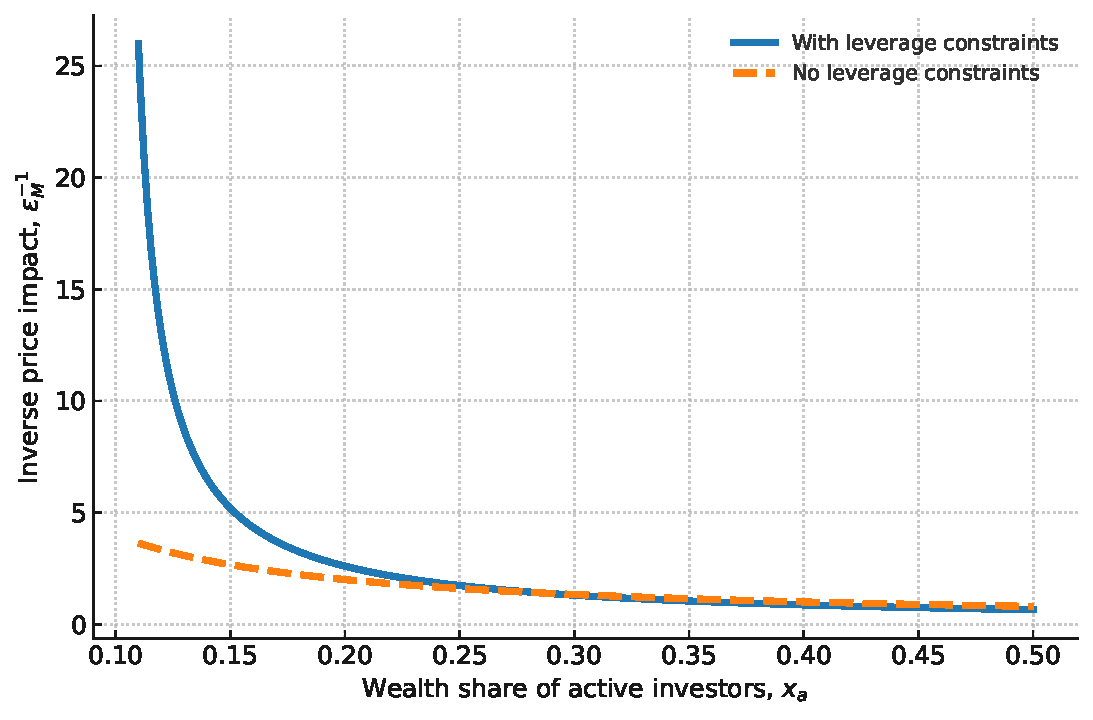
\includegraphics[width=\linewidth]{figures/price_impact_lev_constraints1.pdf}
        \caption{Role of leverage constraints \emph{(assumes $x_{c,t}=0.10$)}}
        % \label{fig:impact_het_vs_hom}
    \end{subfigure}\hfill
    % --- Right: price impact vs x_c for fixed x_a ---
    \begin{subfigure}[t]{0.48\textwidth}
        \centering
        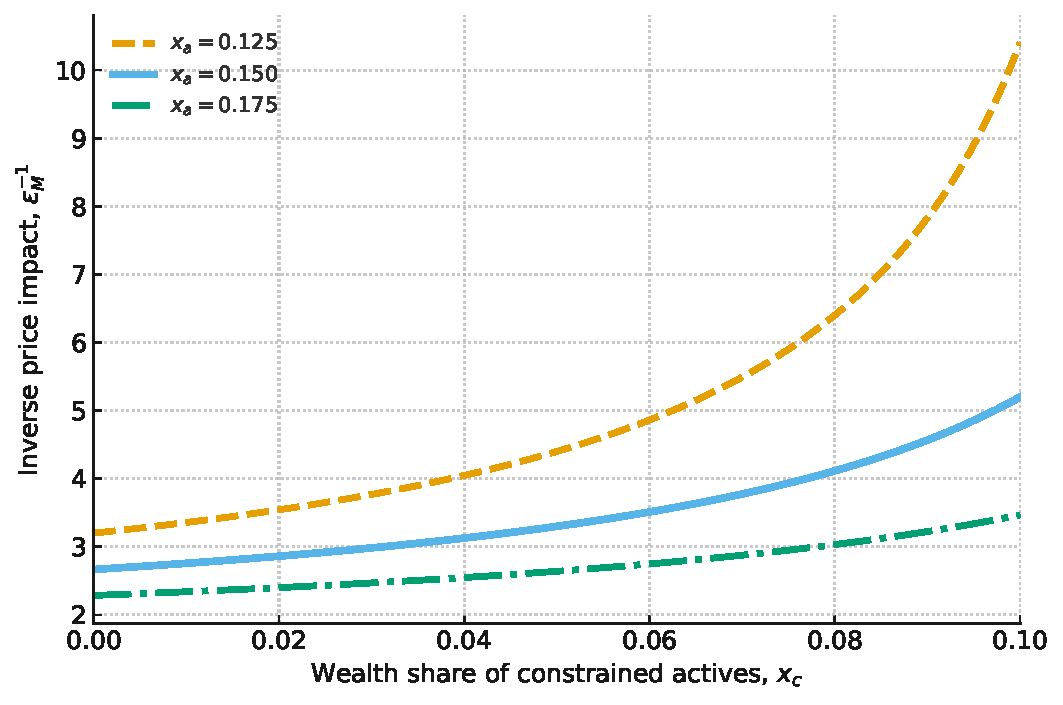
\includegraphics[width=\linewidth]{figures/price_impact_lev_constraints2.pdf}
        \caption{Varying the wealth share of constrained actives, $x_{c,t}$}
        % \label{fig:impact_vs_w1_by_alphap}
    \end{subfigure}
    \vspace{2mm}
    \caption{Price impact under leverage constraints. Panel (a) compares the cases with and without leverage constraints (holding $x_{c,t}=0.10$). Panel (b) plots the price impact as a function of $x_{c,t}$ for different values of $x_{a,t}$.}
    \label{fig:price_impact_leverage_constraints}
\end{figure}

% \paragraph{Taking stock.}
% Proposition~\ref{prop_elasticity_pref_heterog} enables us to characterize several key features of the aggregate market elasticity. First, the elasticity is \emph{finite} when risk is misallocated in the economy: small portfolio flows around a frictionless allocation have no first-order price impact. Second, preference heterogeneity tends to amplify price impact in bad times. As the wealth share of active investors falls, the efficient portfolio share of passive investors rises, widening the gap between efficient and actual portfolios. Third, leverage constraints further amplify price impact in bad times by shrinking $x_{u,t}$, the wealth share of marginal (unconstrained) investors. Therefore, aggregate market elasticity \emph{displays} rich state dependence in economies with heterogeneous investors and financial frictions.
\paragraph{Taking stock.}
Proposition~\ref{prop_elasticity_pref_heterog} clarifies the main determinants of aggregate market elasticity. The elasticity is \emph{finite} only when risk is misallocated: small portfolio flows around the frictionless allocation have no first-order price impact. Preference heterogeneity amplifies price impact in downturns because, as the active wealth share falls, the efficient passive share rises, widening the gap between efficient and actual portfolios. Binding leverage constraints further increase price impact by shrinking the marginal (unconstrained) risk-bearing capacity, $x_{u,t}$. Taken together, these forces imply rich state dependence of aggregate elasticity in economies with heterogeneous investors and financial frictions.



% The right panel of Figure~\ref{fig:price_impact_comparison} highlights the role of the wealth distribution among active investors. 
% Assuming $J = 2$ and $\gamma_1 > \gamma_2$, the average risk aversion among active investors is given by $\mathbb{E}^u[\gamma_j] = w_1 \gamma_1 + (1-w_1) \gamma_2$, where $w_1 = \frac{x_1}{x_a}$. 
% The figure shows that the price impact increases as the share of the more risk-averse active investor increases. 
% The reason is that as the average risk aversion of active investors increases, the passive investor should optimally hold more of the risky asset. 
% If the passive investor does not adjust its portfolio, this would worsen the allocation of risk, raising the price impact. 



% Several points are worth emphasizing. First, note that with heterogeneous active investors even in the case in which $ \overline{\alpha}_p=1 $, the aggregate elasticity is finite. As we show later in the next section, this effect is due to impact of flows on the risk-free rate. %\textcolor{red}{We probably need to say more here.}

% Second, assuming that the passive agents are more risk-averse than active investors, that is $ \gamma_{0}\ge\mathbb{E}^{u}[\gamma_{j}] $, with $ \psi>1 $, introducing preference heterogeneity attenuates the price response to flows, leading to more elastic markets relative to the economy without heterogeneity in Proposition~\ref{prop:elasticity_passive_demand}. This result is due to risk misallocation, as passive investors are effectively closer to their optimal portfolio when $\gamma_0  > \mathbb{E}^u[\gamma_j]$, for a given initial value $\overline{\alpha}_p < 1$.
% To see this point, let's compute the optimal portfolio share that investor $j = 0$ would choose if she was an active investor:
% % : for a given active wealth distribution $ x_a $, more risk-averse passive investors demand a higher risk premium for holding extra units of the risky asset, leading to a more depressed asset price response to flows.
% \begin{equation}
%     \overline{\alpha}_p^{optimal} = 1- x_a \left[ \frac{\gamma_0 - \mathbb{E}^a[\gamma_j]}{\gamma} \right],
% \end{equation}
% If type $j = 0$ investors have high risk aversion, then it is optimal for them to invest less than 100$\%$ in the risky asset. In this case, $\overline{\alpha}_p < 1$ is not an indication of risk misallocation, but it reflects the optimal risk sharing among investors. 
% It turns out that the elasticity will be positive if $\alpha_p < \overline{\alpha}_p^{optimal}$:
% \begin{equation}
% 	\varepsilon_M^{-1}=\left(1-\psi^{-1}\right) \frac{\gamma \sigma^{2}}{y_{0}(X)}\frac{\overline{\alpha}_{p,t}^{optimal}-\overline{\alpha}_{p}}{x_{a}}+\mathcal{O}\left(\epsilon^{2}\right).
% 	\end{equation}
% This shows that risk misallocation is again the key ingredient necessary to obtain a finite elasticity. Notice that a reduction in the wealth share of active investors raises the price impact by more in the presence of heterogeneous preferences, everything else constant. The reason is that a reduction in $x_a$ now raises the optimal portfolio share of passive investors. 
% Optimal risk sharing implies they should hold more of the risky asset when $x_a$ is low, which is typically after a negative aggregate shock. For a given level of $\overline{\alpha}_p$, this implies that there is more risk misallocation when $x_a$ is low, that is, $\overline{\alpha}_p$ is further away from the optimal.




% Finally, from Equation~\eqref{eq:elasticity_pref_heterog}, we see that the price impact of flows depends not only on the wealth share of active investors $ x_a $ as before, but also on the wealth distribution among active investors through $ \E^u[\gamma_j] $. This results reiterates the importance of heterogeneity among financial intermediaries that active investors in our model represent (e.g., \citealp{Veronesi/2019};  \citealp{Kargar/2021}). 
% % Also as before, in states in which active investors are undercapitalized, the aggregate market become more inelastic.

% In Figure~\ref{Fig:elasticity_pref_het}, we plot inverse aggregate elasticity for the case with one passive and two active investors ($ J=3 $) with $ \gamma_{0}\ge\gamma_{1}>\gamma_{2} $. In this economy, the two key state variables are the wealth share of active investors, $ x_a $, and the wealth share the most risk-tolerant active investor (agent 2) among active investors, $ w $:
% \begin{equation}\label{eq:state-vars-3agents}
% x_a=1-x_0,\qquad w=\frac{x_2}{x_a}.
% \end{equation}
% \begin{figure}[!t]
% 	\centering
% 	
\includegraphics[width=\textwidth]{./figures/elasticity_heterog.pdf}
% 	\caption{Price impact: passive demand and preference heterogeneity.}
% 	\label{Fig:elasticity_pref_het}
% \end{figure}
% From Figure~\ref{Fig:elasticity_pref_het}, we see that as the active investors become less capitalized and $ x_a $ declines, market become more inelastic. Moreover, as less risk averse active investors become less capitalized and $ w $ goes down, we see a larger price impact from passive flows. 
% %\begin{itemize}
% %	\item Discuss connections with \cite{garleanu2015young}.
% %	\item \sout{Discuss connection with} \cite{Veronesi/2019}.
% %\end{itemize}

% \subsection{Leverage constraints}

% % We consider next the case where investors have heterogeneous preferences and they are subject to leverage constraints. 
% % In Proposition~\ref{prop:elasticity_leverage_constraint}, we derive the aggregate market elasticity when heterogeneous active investors also face leverage constraints.
% % \begin{prop}[Aggregate elasticity: leverage constraints]\label{prop:elasticity_leverage_constraint}
% % 	Suppose $\rho>\left(1-\psi^{-1}\right)\left( \mu - \frac{\gamma\|\sigma\|^2}{2}  \right)$. When active investors have heterogeneous preferences and also face leverage constraints in \eqref{eq:leverage_constraint}, the inverse aggregate market elasticity, $ 1/\varepsilon_M $, is given by:
% % 	%\begin{small}
% % 		\begin{align}		
% % 		\varepsilon_M^{-1}&=
% % 		\left(1-\psi^{-1}\right) \frac{\gamma \sigma^{2}}{y_{0}(X)}\left[\frac{(1-x_c)(1-\overline{\alpha}_{p})}{x_{u}}-\frac{\gamma_{0}-\mathbb{E}^{u}[\gamma_{j}]}{\gamma} -\frac{x_c(\frac{\overline{\sigma}}{\sigma}-1)}{x_u}\right]
% % 		%\left(1-\psi^{-1}\right) \frac{\gamma \sigma^{2}}{y_{0}(X)}\left[\frac{1-\overline{\alpha}_{p}}{x_{u}}-\frac{\gamma_{0}-\mathbb{E}^{u}\left[\gamma_{j}\right]}{\gamma}\right] \nonumber\\
% % 		+\mathcal{O}\left(\epsilon^{2}\right).	\label{eq:elasticity_leverage_constraint}		
% % 		%&+\left(1-\psi^{-1}\right) \frac{\gamma \sigma^{2}}{y_{0}(X)}\left[\frac{\mathbb{E}^{u}\left[\gamma_{k}\right]-\mathbb{E}^{c}\left[\gamma_{k}\right]}{\gamma x_{u}}+\frac{\gamma \sigma\left(1-\psi^{-1}\right)}{2 y_{0}(X)} \frac{\gamma_{0}-\mathbb{E}^{u}\left[\gamma_{k}\right]}{\gamma}+\frac{\overline{\alpha}_{p}-\frac{\overline{\sigma}}{\sigma}}{x_{u}}\right] x_{c}+\mathcal{O}\left(\epsilon^{2}\right),	\label{eq:elasticity_leverage_constraint}		
% % 		\end{align}						
% % 	%\end{small}		
% % \end{prop}
% % \begin{proof}
% % 	See Appendix~\ref{app:prop_elasticity_leverage_constraint}.
% % \end{proof}
% % We highlight several points from Proposition~\ref{prop:elasticity_leverage_constraint}. First, note than when all active agents are unconstrained, i.e., $ x_c=0 $, we get the price impact from Proposition~\ref{prop_elasticity_pref_heterog}. Similar to the case with heterogeneous investors, the aggregate elasticity is finite when $ \overline{\alpha}_p=1 $.



% % \begin{figure}[!t]
% % 	\centering
% % 	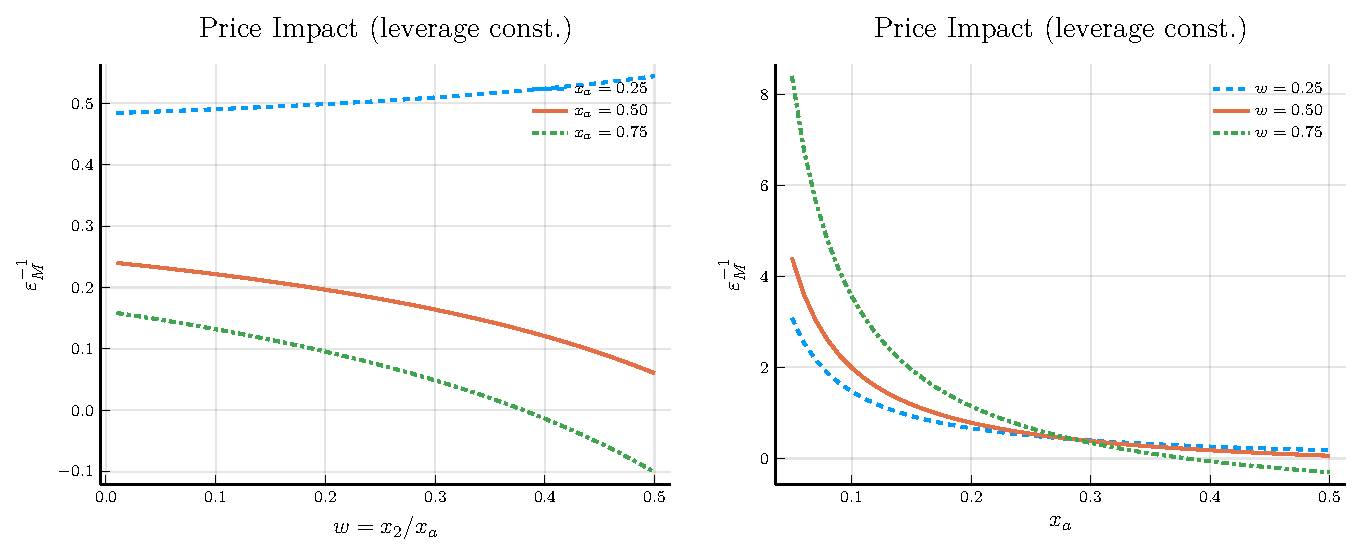
\includegraphics[width=\textwidth]{figures/elasticity_lev-const.pdf}
% % 	\caption{Price impact: leverage constraints.}
% % 	\label{Fig:elasticity_leverage_const}
% % \end{figure}

% As in the previous two cases, risk misallocation plays an important role. The optimal portfolio share of type $j = 0$ investors, i.e. the portfolio they would choose if they were active, is given by
% \begin{equation}
%     \overline{\alpha}_{p,t}^{\mathrm{opt}} = 1 -\frac{x_u}{1-x_c}\frac{\gamma_0-\mathbb{E}^u[\gamma_j] }{\gamma} - \frac{x_c(\frac{\overline{\sigma}}{\|\sigma\|}-1)  }{1-x_c}.
% \end{equation}
% Plugging the formula for the optimal portfolio share in the expression for the aggregate market elasticity, we obtain
% \begin{equation}
% 	\varepsilon_M^{-1}=\left(1-\psi^{-1}\right) \frac{\gamma \sigma^{2}}{y_{0}(X)}\frac{\overline{\alpha}_{p,t}^{\mathrm{opt}}-\overline{\alpha}_{p}}{x_{a}}(1-x_c)+\mathcal{O}\left(\epsilon^{2}\right).
% 	\end{equation}
% As before, the market elasticity is finite and positive when $\overline{\alpha}_p$ is below its optimal level. The optimal portfolio now depends on the average risk aversion of unconstrained agents, the leverage constraint, and the entire distribution among active investors. 
% Figure~\ref{Fig:elasticity_frictions} illustrates the behavior of the market elasticity in the presence of leverage constraints. The left panel shows the price impact for different values of $w = x_2/x_a$, that is, the share of wealth of the low risk aversion investor among active investors. 
% The right panel shows the inverse elasticity as a function of the wealth share of active investors. 


% % Let us consider an example to help simplify the exposition. Suppose there are three agents ($ J=3 $), one passive and two active investors, with risk aversions $ \gamma_{0}=\gamma_1>\gamma_2 $. As before, $ j=0 $ represents the passive investor. For simplicity, also assume $ \overline{\alpha}_p=1 $ and $ \overline{\sigma}=\sigma $. First, suppose agent 2 is unconstrained, so that $ x_u=x_1+x_2 $ and $ x_c=0 $. In this case, only the second term in the square bracket in Equation~\eqref{eq:elasticity_leverage_constraint} is non-zero, leading to a \textit{negative} price impact of the asset flows:
% % \[\epsilon_M^{-1}=
% % -\left(1-\psi^{-1}\right)\frac{\gamma\sigma^2}{y_0(X)}\frac{\gamma_0-\E^u[\gamma_{j}]}{\gamma}<0.\]

% % Now suppose agent 2 faces binding leverage constraint, so that  $ x_u=x_1 $, and $ x_c=x_2 $. In this case we have 
% % \[ \E^u\left[\gamma_k\right]=\gamma_{0}>\E^c\left[\gamma_k\right]=\gamma_2.\]
% % Note that, in this case, only the first term in the square bracket in the second line of Equation~\eqref{eq:elasticity_leverage_constraint} is positive and all other terms are zero. So, the inverse aggregate elasticity simplifies to 
% % \[\varepsilon_M^{-1}=\left(1-\psi^{-1}\right) \frac{\left(\gamma_{0}-\gamma_{2}\right)\sigma^2}{y_{0}(X) x_{u}}>0,\]
% % and flows lead to an increase in the price-dividend ratio. Thus, the introduction of the constrained investor leads to a \textit{positive} price response to flows and a finite aggregate elasticity. This result shows that even when passive investors are fully invested in the risky asset, the presence of binding portfolio constraints can lead to finite market elasticity. This is again due to 
% % % \textcolor{red}{needs to be completed $ \dots $}%risk misallocation: when the leverage constraint binds to investor 2, the more risk averse need to have higher 

% \begin{figure}[!t]
% 	\centering
% 	
\includegraphics[width=\textwidth]{figures/elasticity_frictions.pdf}
% 	\caption{Decomposition of the inverse aggregate market elasticity.}
% 	\label{Fig:elasticity_frictions}
% \end{figure}


% %\textcolor{red}{
% %\begin{itemize}
% %	\item Need to dissect the extra term from leverage constraint. 
% %	\item \sout{Perhaps consider 3 types: one passive with $ \gamma_{0} $, and two active with $ \gamma_0=\gamma_1>\gamma_2 $. For simplicity can also assume $ \overline{\alpha}_p=1 $ and $ \overline{\sigma}=\sigma $.}
% %	\item \sout{To get intuition, look at components of elasticity separately: $ \dfrac{\partial\eta_2}{\partial F} $ and $ \dfrac{\partial r_2}{\partial F} $.}
% %	\item \sout{look at the impact of flows on the risk premium $\eta\sigma$. This has three components. $r$, risk premium, and volatility.}
% %	\item \sout{would like to see the response of risk premium}
% %	\item also response of volatility
% %\end{itemize}}
% %\begin{prop}\label{prop:elasticity_second_order}
% %	The inverse aggregate market elasticity $ 1/\varepsilon_M $ is given under the following three conditions:
% %	\begin{enumerate}[(i)]
% %		\item \textbf{Passive demand:} If there is no preference heterogeneity and active investors do not face leverage constraint, the inverse elasticity is given by:
% %		\[\frac{1}{p(X, \epsilon)} \frac{\partial p(X, \epsilon)}{\partial F(X, \epsilon)}=\left(1-\psi^{-1}\right) \frac{\gamma \sigma^{2}}{y_{0}(X)} \frac{1-\bar{\alpha}_{p}}{x_{1}}+\mathcal{O}\left(\epsilon^{2}\right).\]
% %		\item \textbf{Preference heterogeneity:} If active investors have heterogeneous risk aversions but face no leverage constraint, the inverse elasticity is given by:
% %		\[\frac{1}{p(X, \epsilon)} \frac{\partial p(X, \epsilon)}{\partial F(X, \epsilon)}=\left(1-\psi^{-1}\right) \frac{\gamma \sigma^{2}}{y_{0}(X)}\left[\frac{1-\bar{\alpha}_{p}}{x_{a}}-\frac{\hat{\gamma}_{0}-\mathbb{E}^{u}\left[\hat{\gamma}_{j}\right]}{\gamma}\right]+\mathcal{O}\left(\epsilon^{2}\right),\]
% %		where $ \mathbb{E}^u\left[ \hat{\gamma}_j\right] \equiv\sum_{j\in\mathcal{J}^u} \frac{x_j}{x_u} \hat{\gamma}_j, $ and $ x_{a} \equiv 1-x_{0} $ denotes the wealth share of active investors.
% %		\item \textbf{Leverage constraints:} When active investors have heterogeneous preferences and also face leverage constraints, the inverse market elasticity is given by:
% %		\begin{small}
% %			\begin{align*}
% %				\frac{1}{p(X, \epsilon)} \frac{\partial p(X, \epsilon)}{\partial F(X, \epsilon)}&=
% %				\left(1-\psi^{-1}\right) \frac{\gamma \sigma^{2}}{y_{0}(X)}\left[\frac{1-\bar{\alpha}_{p}}{x_{u}}-\frac{\hat{\gamma}_{0}-\mathbb{E}^{u}\left[\hat{\gamma}_{j}\right]}{\gamma}\right] \\
% %				&+\left(1-\psi^{-1}\right) \frac{\gamma \sigma^{2}}{y_{0}(X)}\left[\frac{\mathbb{E}^{u}\left[\hat{\gamma}_{k}\right]-\mathbb{E}^{c}\left[\hat{\gamma}_{k}\right]}{\gamma x_{u}}+\frac{\gamma \sigma\left(1-\psi^{-1}\right)}{2 y_{0}(X)} \frac{\gamma_{0}-\mathbb{E}^{u}\left[\hat{\gamma}_{k}\right]}{\gamma}+\frac{\bar{\alpha}_{p}-\frac{\bar{\sigma}}{\sigma}}{x_{u}}\right] x_{c}\\
% %				&+\mathcal{O}\left(\epsilon^{2}\right),			
% %			\end{align*}						
% %		\end{small}		
% %	where $ \textcolor{red}{\mathbb{E}^c\left[ \hat{\gamma}_k\right] \equiv\sum_{k\in\mathcal{J}^c} \frac{x_k}{x_c} \hat{\gamma}_j.} $
% %	\end{enumerate}
% %\end{prop}
% %\begin{proof}
% %	See Appendix~\ref{app:prop_second_order_elasticity}.
% %\end{proof}

% %\begin{itemize}
% %    \item \sout{Define flows}
% %    \item \sout{Show opposite effects on interest rate and risk premium}
% %    \item \sout{Infinite elasticity up to first-order}
% %    \item \sout{You need to go to second-order}
% %    \item \sout{Three cases in second-order}
% %    \begin{itemize}
% %        \item \sout{Passive investment / risk concentration}
% %        \item \sout{Heterogeneity}
% %        \item \sout{Leverage constraints}
% %    \end{itemize}
% %	\item Discussion of Prop 2    
% %\end{itemize}

% % \section{Aggregate Elasticity and Excess Volatility}
% % \begin{itemize}
% % 	\item Quantitative implications
% % 	\begin{itemize}
% % 		\item Connection between volatility and elasticity
% % 	\end{itemize}
	
% % 	\begin{equation}
% % 		\sigma_p(x,\overline{\alpha}_p) = \frac{p_x}{p} \sigma_x + \frac{p_{\overline{\alpha}_p}}{p} \sigma_{\overline{\alpha}_p}
% % 	\end{equation}
	
	
% % 	\begin{equation}
% % 		\frac{d p}{p} = \frac{1}{\varepsilon_M(X)} dF
% % 	\end{equation}
	
% % \end{itemize}
% % In Proposition~\ref{prop:volatility-flow}, we assess the impact of flows on return volatility $ \sigma_{R} $.
% % \begin{prop}[Portfolio flows and volatility]\label{prop:volatility-flow}
% % 	The impact of asset flows on return volatility is
% % 	\begin{equation}\label{eq:volatility-flow}
% % 		\frac{\partial\sigma_{R}(X,\epsilon)}{\partial F(X,\epsilon)}=-\left(1-\psi^{-1}\right) \frac{\gamma \sigma^{2}}{2 y_{0}(X)}\sigma\left(\hat{\gamma}_{0}-\mathbb{E}^{u}\left[\hat{\gamma}_{k}\right]\right)
% % 	\end{equation}
% % \end{prop}
% % We used $ \sigma_{R,1}(X)=0 $ and $ \sigma_{R,2}(X)=-\sigma_{y,2}(X). $
% % \begin{proof}
% % 	See Appendix~\ref{app:prop_volatility-flow}.
% % \end{proof}

% % \section{Discussion and Main Lessons}
% % We draw four main lessons from the results in Propositions~\ref{prop:elasticity_passive_demand}--\ref{prop:volatility-flow}.
% % \begin{lesson}[The role of interest rates]
% % 	Regardless of how constrained agents are, in the unit EIS case ($ \psi=1 $), the aggregate market elasticity is infinite. 
% % \end{lesson}
% % We need $ \psi>1 $ to obtain positive price impact of flow shocks.

% % \begin{lesson}[State dependence]
% % 	The aggregate elasticity is time-varying and state-dependent.
% % \end{lesson}
% % Market elasticity is function of economy's aggregate sate variables, capturing time-varying investment opportunities. 

% % \begin{lesson}[Risk misallocation]
% % 	Markets are inelastic when risk is misallocated in the economy.
% % \end{lesson}
% % Conjecture: with perfect risk sharing, there is no price impact.

% % \begin{lesson}[Volatility]
% % 	Volatility depends on both market elasticity and portfolio flow shocks.
% % \end{lesson}





% % \section{Decomposition of the Aggregate Market Elasticity}
% % Equipped with the definition of (inverse) market elasticity in Equation~\eqref{eq:elasticity-y2}, we can use the pricing condition in \eqref{eq:pricing_cond} to decompose the price impact into three terms: the impact of flows on (i) the risk-free rate, (ii) the risk-premium, and (iii) the drift of the asset price. This decomposition is given by
% % \begin{equation}\label{eq:elasticity-decomp}
% % 	\varepsilon_M^{-1}=-\frac{1}{y_0(X)}\left[\frac{\partial r_2(X)}{\partial\hat{\alpha}_p}+
% % 	\frac{\partial\pi_2(X)}{\partial\hat{\alpha}_p}-
% % 	\frac{\partial\mu_{P,2}(X)}{\partial\hat{\alpha}_p}\right]\frac{\epsilon}{x_0},
% % \end{equation}
% % where $ \mu_{P,t}=\mu-\mu_{y,t}-\sigma_{y,t}\sigma_{R,t} $ is the drift of the risky asset price $ P_t $, and $ \pi_t=\sigma_{R,t}\eta_t $ is the risk premium. The second-order correction for the risk premium and the asset price drift can be derived easily:
% % \begin{align}
% % 	\pi_{2}(X)&=-\eta_{0}(X) \sigma_{y, 2}(X)+\eta_{2}(X) \sigma\\
% % 	\mu_{P,2}(X)&=-\mu_{y,2}(X)-\sigma\sigma_{y,2}(X),
% % \end{align}
% % where we use the fact that $ \sigma_{y,0}(X)=\sigma_{R,0}(X)=\sigma_{y,1}(X)=\sigma_{R,1}(X)=0 $. We again consider the three cases we discussed in the previous section.

% % \begin{figure}[!t]
% % 	\centering
% % 	
\includegraphics[width=\textwidth]{./figures/p_impact_het_decomp.pdf}
% % 	\caption{Decomposition of the inverse aggregate market elasticity.}
% % 	\label{Fig:elasticity_decomp}
% % \end{figure}
% % \textcolor{red}{discuss the interpretation of the three terms: interest rate, risk premium, and drift of the price.}


% % \subsection{Passive demand}
% % In the absence of investor heterogeneity (i.e., $ \hat{\gamma}_j=0 $ for all $ j $) and leverage constraints (that is $ x_c=0 $), we have $ \mu_{P,2}(X)=-\mu_{y,2}(X)=0 $. In this case, $ \sigma_{y, 2}(X)=\eta_{2}(X)=0 $ and therefore, $ \pi_2(X)= 0$. Thus, we have $ r_2(X)=y_2(X) $ and  
% % \begin{align*}
% % 	\frac{\partial\mu_{P,2}(X)}{\partial\hat{\alpha}_p}=0,
% % 	\qquad\frac{\partial\pi_{2}(X)}{\partial\hat{\alpha}_p}=0,
% % 	\qquad\frac{\partial r_{2}(X)}{\partial\hat{\alpha}_p}=\frac{\partial y_{2}(X)}{\partial\hat{\alpha}_p}.
% % \end{align*}
% % Therefore, the aggregate elasticity is
% % \[\varepsilon_M^{-1}=-\frac{1}{y_0(X)}\frac{\partial r_2(X)}{\partial \hat{\alpha}_p}\frac{\epsilon}{x_0}=
% % \left(1-\psi^{-1}\right) \frac{\gamma \sigma^{2}}{y_{0}(X)} \frac{1-\overline{\alpha}_{p}}{x_{a}}+\mathcal{O}\left(\epsilon^{2}\right)\]
% % which is exactly the expression for the aggregate market elasticity in Proposition~\ref{prop:elasticity_passive_demand}. 

% % So, in the case where all investors have the same preferences and do not face leverage constraints, the market elasticity is entirely determined by the second-order impact of flows on the risk-free rate.

% % \textcolor{red}{mention everyone has the same risk aversion.}

% % \subsection{Investor heterogeneity}
% % In this case, the impact of flows can be summarized as
% % \begin{small}
% % 	\begin{align*}
% % 		-\frac{\partial\mu_{P,2}(X)}{\partial\hat{\alpha}_p}\frac{\epsilon}{x_0}&=\left(1-\psi^{-1}\right)\frac{\gamma\sigma^2}{2y_0(X)}(\gamma-1)\sigma^2\left(\frac{\gamma_{0}-\mathbb{E}^{u}\left[\gamma_{j}\right]}{\gamma}\right)
% % 		+\left(1-\psi^{-1}\right)\frac{\gamma \sigma^{2}}{2 y_{0}(X)}\sigma^2\left(\frac{\gamma_{0}-\mathbb{E}^{u}\left[\gamma_{j}\right]}{\gamma}\right),\\
% % 		\frac{\partial\pi_{2}(X)}{\partial\hat{\alpha}_p}\frac{\epsilon}{x_0}&=-\left(1-\psi^{-1}\right) \frac{\gamma \sigma^{2}}{2 y_{0}(X)}(1+\gamma)\sigma^2\left(\frac{\gamma_{0}-\mathbb{E}^{u}\left[\gamma_{j}\right]}{\gamma}\right)-\frac{\gamma\sigma^2}{x_a}\E^u[\hat{\gamma}_j]\epsilon,\\
% % 		\frac{\partial r_{2}(X)}{\partial\hat{\alpha}_p}\frac{\epsilon}{x_0}&=
% % 		-\left(1-\psi^{-1}\right)\frac{\gamma\sigma^2}{2y_0(X)}(\gamma-1)\sigma^2\left(\frac{\gamma_{0}-\mathbb{E}^{u}\left[\gamma_{j}\right]}{\gamma}\right)
% % 		-\left(1-\psi^{-1}\right)\gamma\sigma^2\left[\frac{1-\overline{\alpha}_{p}}{x_{a}}-\frac{\gamma_{0}-\mathbb{E}^{u}\left[\gamma_{j}\right]}{\gamma}\right]\\
% % 		&\quad+\left(1-\psi^{-1}\right)\frac{\gamma \sigma^{2}}{2 y_{0}(X)}\gamma\sigma^2\left(\frac{\gamma_{0}-\mathbb{E}^{u}\left[\gamma_{j}\right]}{\gamma}\right)+\frac{\gamma\sigma^2}{x_a}\E^u[\hat{\gamma}_j]\epsilon.
% % 	\end{align*}
% % \end{small}
% % \textcolor{red}{Discuss the intuition.}

% % \subsection{Leverage constraints}
% % In this case, the impact of flows can be summarized as
% % \begin{small}
% % 	\begin{align*}
% % 		-\frac{\partial\mu_{P,2}(X)}{\partial\hat{\alpha}_p}\frac{\epsilon}{x_0}&=\left(1-\psi^{-1}\right)\frac{\gamma\sigma^2}{2y_0(X)}(\gamma-1)\sigma^2\left(\frac{\gamma_{0}-\mathbb{E}^{u}\left[\gamma_{j}\right]}{\gamma}\right)
% % 		+\left(1-\psi^{-1}\right)\frac{\gamma \sigma^{2}}{2 y_{0}(X)}\sigma^2\left(\frac{\gamma_{0}-\mathbb{E}^{u}\left[\gamma_{j}\right]}{\gamma}\right),\\
% % 		\frac{\partial\pi_{2}(X)}{\partial\hat{\alpha}_p}\frac{\epsilon}{x_0}&=
% % 		-\left(1-\psi^{-1}\right) \frac{\gamma \sigma^{2}}{2 y_{0}(X)}\left(\gamma+\frac{(1-\gamma)x_c+1-x_0}{x_u}\right)\sigma^2\left(\frac{\gamma_{0}-\mathbb{E}^{u}\left[\gamma_{j}\right]}{\gamma}\right)-\frac{\gamma\sigma^2}{x_a}\E^u[\hat{\gamma}_j]\epsilon,\\
% % 		\frac{\partial r_{2}(X)}{\partial\hat{\alpha}_p}\frac{\epsilon}{x_0}&=
% % 		-\left(1-\psi^{-1}\right)\frac{\gamma\sigma^2}{2y_0(X)}(\gamma-1)\sigma^2\left(\frac{\gamma_{0}-\mathbb{E}^{u}\left[\gamma_{j}\right]}{\gamma}\right)\\
% % 		&\quad-\left(1-\psi^{-1}\right)\gamma\sigma^2\left[\frac{1-\overline{\alpha}_{p}}{x_{a}}-\frac{\gamma_{0}-\mathbb{E}^{u}\left[\gamma_{j}\right]}{\gamma}\right]\\
% % 		&\quad-\left(1-\psi^{-1}\right) \frac{\gamma \sigma^{2}}{y_{0}(X)}\left[\frac{\mathbb{E}^{u}\left[\gamma_{k}\right]-\mathbb{E}^{c}\left[\gamma_{k}\right]}{\gamma x_{u}}+\frac{\gamma \sigma\left(1-\psi^{-1}\right)}{2 y_{0}(X)} \frac{\gamma_{0}-\mathbb{E}^{u}\left[\gamma_{k}\right]}{\gamma}+\frac{\overline{\alpha}_{p}-\frac{\overline{\sigma}}{\sigma}}{x_{u}}\right] x_{c}\\
% % 		&\quad+\left(1-\psi^{-1}\right)\frac{\gamma \sigma^{2}}{2 y_{0}(X)}\left(\gamma+\frac{(1-\gamma)x_c+x_c}{x_u}\right)\sigma^2\left(\frac{\gamma_{0}-\mathbb{E}^{u}\left[\gamma_{j}\right]}{\gamma}\right)+\frac{\gamma\sigma^2}{x_a}\E^u[\hat{\gamma}_j]\epsilon.
% % 	\end{align*}
% % \end{small}
% % \textcolor{red}{Discuss the intuition.}

        
% % \section{Price impact and risk misallocation}

% % \paragraph{No leverage constraints.} Assume there is no leverage constraints. Investor $j$'s demand for risk, for $j = 1,\ldots, J$, is given by 
% % \begin{equation}
% %     \sigma_j(X) = \sigma + \sigma \left[  \sum_{k=1}^J \frac{x_k}{1-x_0} \hat{\gamma}_k - \hat{\gamma}_j  - \frac{\hat{\alpha}_p x_0}{1-x_0}\right] \epsilon + \mathcal{O}(\epsilon^2).
% % \end{equation}

% % Therefore, if investor $j = 0$ were active (i.e., $x_0=0$), the optimal risk allocation would satisfy:
% % \begin{equation}
% %     \sigma_j(X) = \sigma + \sigma \left[  \sum_{k=0}^J x_k \hat{\gamma}_k - \hat{\gamma}_j  \right] \epsilon + \mathcal{O}(\epsilon^2).
% % \end{equation}

% % The passive investor's actual risk exposure is given by $\sigma_0(X) = \sigma + \hat{\alpha}_p \sigma \epsilon$. Hence, the actual risk exposure coincides with the optimal risk exposure if
% % \begin{align}
% %     \hat{\alpha}_p^{optimal} &=  \sum_{k=1}^J x_k \hat{\gamma}_k - (1-x_0) \hat{\gamma}_0 \\
% %     &= - x_a \left[ \frac{\gamma_0 - \mathbb{E}^a[\gamma_j]}{\gamma} \right],
% % \end{align}
% % where $\mathbb{E}^a[\gamma_j] \equiv \sum_{k=1}^J \frac{x_k}{1-x_0} \gamma_k$ and $x_a\equiv(1-x_0)$.

% % The price impact with heterogeneous preferences is given by
% % \begin{equation}
% % 	%\frac{1}{p(X, \epsilon)} \frac{\partial p(X, \epsilon)}{\partial F(X, \epsilon)}
% % 	\varepsilon_M^{-1}=\left(1-\psi^{-1}\right) \frac{\gamma \sigma^{2}}{y_{0}(X)}\left[\frac{1-\overline{\alpha}_{p}}{x_{a}}-\frac{\gamma_{0}-\mathbb{E}^{a}[\gamma_{j}]}{\gamma}\right]+\mathcal{O}\left(\epsilon^{2}\right),
% % \end{equation}

% % Using the fact that $\overline{\alpha}_p = 1 + \hat{\alpha}_p \epsilon$ and $x_a = 1-x_0$, we obtain that the price impact is given by
% % \begin{equation}
% % 	%\frac{1}{p(X, \epsilon)} \frac{\partial p(X, \epsilon)}{\partial F(X, \epsilon)}
% % 	\varepsilon_M^{-1}=\left(1-\psi^{-1}\right) \frac{\gamma \sigma^{2}}{y_{0}(X)}\left[-\frac{\hat{\alpha}_{p}}{1-x_0}-\frac{\gamma_{0}-\mathbb{E}^{a
% %  }[\gamma_{j}]}{\gamma}\right]+\mathcal{O}\left(\epsilon^{2}\right) \approx 0.
% % \end{equation}

% % Notice that we can write the price impact as follows:
% % \begin{equation}
% % 	%\frac{1}{p(X, \epsilon)} \frac{\partial p(X, \epsilon)}{\partial F(X, \epsilon)}
% % 	\varepsilon_M^{-1}=\left(1-\psi^{-1}\right) \frac{\gamma \sigma^{2}}{y_{0}(X)}\frac{\overline{\alpha}_p^{opt}-\overline{\alpha}_{p}}{x_{a}}+\mathcal{O}\left(\epsilon^{2}\right),\label{eq:price-impact-het-misallocation}
% % \end{equation}

% % \paragraph{Leverage constraints.} With leverage constraints, the risk exposure is given by
% % \begin{equation}
% %     \sigma_j(X) = \sigma_{j,0}(X) +\|\sigma\|\min\left\{ \sum_{k\in\mathcal{J}^u} \frac{x_k}{x_u} \hat{\gamma}_k -\left(\frac{\hat{\alpha}_p  x_0+\frac{\hat{\sigma}}{\|\sigma\|} x_c }{1-x_0-x_c}\right)- \hat{\gamma}_j  ,\frac{\hat{\sigma}}{\|\sigma\|}  \right\}\epsilon + \mathcal{O}(\epsilon^2).
% % \end{equation}

% % This reflects the effects of two frictions: leverage constraints and the presence of passive investors. To isolate the role of each friction, assume there is no passive investors, so the risk exposure is given by 
% % \begin{equation}
% %     \sigma_j(X) = \sigma_{j,0}(X) +\|\sigma\|\min\left\{ \sum_{k=0}^{J_u} \frac{x_k}{1-x_c} \hat{\gamma}_k -\frac{\frac{\hat{\sigma}}{\|\sigma\|} x_c }{1-x_c}- \hat{\gamma}_j  ,\frac{\hat{\sigma}}{\|\sigma\|}  \right\}\epsilon + \mathcal{O}(\epsilon^2),
% % \end{equation}
% % where we assume that investors $j \in \{0, 1,\ldots, J_u\}$ are unconstrained given the current state.

% % Investor $j$ would be holding his privately optimal portfolio if
% % \begin{align}
% %     \hat{\alpha}_p^{opt} \epsilon &= \left[\sum_{k=0}^{J_u} \frac{x_k}{1-x_c} \hat{\gamma}_k -\frac{\frac{\hat{\sigma}}{\|\sigma\|} x_c }{1-x_c}- \hat{\gamma}_0\right] \epsilon\\
% %      &= -\frac{x_u}{1-x_c}\frac{\gamma_0-\mathbb{E}^u[\gamma_j] }{\gamma} - \frac{\frac{\hat{\sigma}}{\|\sigma\|} x_c }{1-x_c},
% % \end{align}
% % where $x_u=1-x_c - x_0.$
% % The price impact is given by
% % \begin{align}		
% % 		\varepsilon_M^{-1}&=
% % 		\left(1-\psi^{-1}\right) \frac{\gamma \sigma^{2}}{y_{0}(X)}\left[\frac{(1-x_c)(1-\overline{\alpha}_{p})-x_c(\frac{\overline{\sigma}}{\sigma}-1)}{1-x_c -x_0}-\frac{\gamma_{0}-\mathbb{E}^{u}[\gamma_{j}]}{\gamma}\right]%\nonumber\\
% % 		%\left(1-\psi^{-1}\right) \frac{\gamma \sigma^{2}}{y_{0}(X)}\left[\frac{1-\overline{\alpha}_{p}}{x_{u}}-\frac{\gamma_{0}-\mathbb{E}^{u}\left[\gamma_{j}\right]}{\gamma}\right] \nonumber\\
% % 	%	&+\left(1-\psi^{-1}\right) \frac{\gamma \sigma^{2}}{y_{0}(X)}\left[\frac{\mathbb{E}^{u}[\gamma_{k}]-\mathbb{E}^{c}[\gamma_{k}]}{\gamma x_{u}}+\frac{\gamma \sigma\left(1-\psi^{-1}\right)}{2 y_{0}(X)} \frac{\gamma_{0}-\mathbb{E}^{u}[\gamma_{k}]}{\gamma}\right] x_{c}
% %   +\mathcal{O}\left(\epsilon^{2}\right),		
% % 		\end{align}						
% % 	%\end{small}		
% % 	where $ \mathbb{E}^c[\gamma_k] \equiv\sum_{k\in\mathcal{J}^c} \frac{x_k}{x_c} \gamma_j. $

% % Plugging the expression for privately optimal $\overline{\alpha}_p$, the first term in bracket cancels out:
% % \begin{align}		
% %     \varepsilon_M^{-1}&= \left(1-\psi^{-1}\right) \frac{\gamma \sigma^{2}}{y_{0}(X)}\left[\frac{\mathbb{E}^{u}[\gamma_{k}]-\mathbb{E}^{c}[\gamma_{k}]}{\gamma x_{u}}+\frac{\gamma \sigma\left(1-\psi^{-1}\right)}{2 y_{0}(X)} \frac{\gamma_{0}-\mathbb{E}^{u}[\gamma_{k}]}{\gamma}\right] x_{c}+\mathcal{O}\left(\epsilon^{2}\right),	
% % \end{align}			


% % \begin{align}		
% %     \varepsilon_M^{-1}&=
% %     \left(1-\psi^{-1}\right) \frac{\gamma \sigma^{2}}{y_{0}(X)}\frac{(1-x_c)(\overline{\alpha}_p^{opt}-\overline{\alpha}_{p})}{x_u}\label{eq:price-impact-lev-misallocation}
% %     %\nonumber\\
% %     %&+\color{blue}{\left(1-\psi^{-1}\right) \frac{\gamma \sigma^{2}}{y_{0}(X)}\left[\frac{\mathbb{E}^{u}[\gamma_{k}]-\mathbb{E}^{c}[\gamma_{k}]}{\gamma x_{u}}+\frac{\gamma \sigma\left(1-\psi^{-1}\right)}{2 y_{0}(X)} \frac{\gamma_{0}-\mathbb{E}^{u}[\gamma_{k}]}{\gamma}\right] x_{c}}
% % 		%\left(1-\psi^{-1}\right) \frac{\gamma \sigma^{2}}{y_{0}(X)}\left[\frac{1-\overline{\alpha}_{p}}{x_{u}}-\frac{\gamma_{0}-\mathbb{E}^{u}\left[\gamma_{j}\right]}{\gamma}\right] \nonumber\\
% % 		% &+\left(1-\psi^{-1}\right) \frac{\gamma \sigma^{2}}{y_{0}(X)}\left[\frac{\mathbb{E}^{u}[\gamma_{k}]-\mathbb{E}^{c}[\gamma_{k}]}{\gamma x_{u}}+\frac{\gamma \sigma\left(1-\psi^{-1}\right)}{2 y_{0}(X)} \frac{\gamma_{0}-\mathbb{E}^{u}[\gamma_{k}]}{\gamma}\right] x_{c}+\mathcal{O}\left(\epsilon^{2}\right),		
% % 		\end{align}		
% % Note that Equation~\eqref{eq:price-impact-het-misallocation} is a special case of Equation~\eqref{eq:price-impact-lev-misallocation} when $x_c=0$ and $x_u=x_a$.

% %   \begin{align}		
% % 		\varepsilon_M^{-1}&=
% % 		\left(1-\psi^{-1}\right) \frac{\gamma \sigma^{2}}{y_{0}(X)}\frac{\overline{\alpha}_p^{opt}-\overline{\alpha}_{p}}{1-\frac{x_0}{1-x_c} } 
% % 		\end{align}		

% % Notice that $\frac{1}{1-\frac{x_0}{1-x_c}}$ is increasing in both $x_0$ and $x_c$. 

% % % \section{Risk misallocation}

% % % \paragraph{Risk misallocation and the aggregate market elasticity.} To better understand how the consumption-wealth ratio may depend on the consumption-wealth ratio, it may be useful to consider a particular specification for the consumption-wealth ratio:
% % % \begin{equation}
% % %     c_j(r, \pi, \overline{\alpha}_p) = \rho \psi + (1-\psi) \left[ r + \pi \overline{\alpha}_j  - \frac{\gamma}{2} \sigma^2 \overline{\alpha}_j^2 \right],
% % % \end{equation}
% % % where $\overline{\alpha}_a$ satisfies the equation $x_a \overline{\alpha}_a + (1-x_a) \overline{\alpha}_p = 1$.

% % % Let $c(r, \pi, \overline{\alpha}_p) = \sum_{j\in\{a,p\}} \omega_j c_j(r, \pi, \overline{\alpha}_p)$ denote the average consumption-wealth ratio. Then, the sensitivity of $c(\cdot)$ with respect to $\overline{\alpha}_p$ is given by
% % % \begin{equation}
% % %     \frac{\partial c(r^*, \pi^*, \overline{\alpha}_p^*)}{\partial \overline{\alpha}_p} = x_a (1-\psi) \left[ \pi^*  - \gamma \sigma^2 \overline{\alpha}_a^*\right] \frac{\partial \overline{\alpha}_a}{\partial \overline{\alpha}_a} + 
% % %     x_p (1-\psi) \left[ \pi^*  - \gamma \sigma^2 \overline{\alpha}_p^*\right].
% % % \end{equation}

% % % If $\overline{\alpha}_j = \frac{\pi^*}{\gamma \sigma^2} $, that is, risk is optimally allocated at the initial equilibrium, then the average consumption-wealth ratio is (locally) independent of $\overline{\alpha}_p$. However, if risk is initially misallocated, then portfolio flows may shift the consumption-wealth ratio schedule depending on whether flows go in the direction of improve or worsen the allocation of risk.

